%\documentclass[envcountsect,envcountsame,runningheads,a4paper]{elsarticle} 
\documentclass[preprint,
    10pt,
%    authoryear,
    3p,
    fleqn,
%    times
]{elsarticle}
%\geometry{margin=2.5cm}
\geometry{top=2cm,bottom=2cm,left=2cm,right=2cm,marginparwidth=1.75cm}

\usepackage{main}

% \allowdisplaybreaks

% Language setting
% Replace `english' with e.g. `spanish' to change the document language
\usepackage[english]{babel}

% Set page size and margins
% Replace `letterpaper' with`a4paper' for UK/EU standard size
% \usepackage[letterpaper,top=2cm,bottom=2cm,left=3cm,right=3cm,marginparwidth=1.75cm]{geometry}

% Useful packages

%\usepackage[colorlinks=true,allcolors=blue]{hyperref}

\begin{document}
\begin{frontmatter}
\title{Probabilistic relations for modelling epistemic and aleatoric uncertainty \\
    its semantics and automated reasoning with theorem proving\tnoteref{t1,t2}}
\tnotetext[t1]{This document is the results of the research project RoboTest (\url{https://robostar.cs.york.ac.uk/}) funded by EPSRC.}
\author[1]{Kangfeng Ye\corref{cor1}}
\ead{kangfeng.ye@york.ac.uk}

\author[1]{Jim Woodcock}
\ead{jim.woodcock@york.ac.uk}

\author[1]{Simon Foster}
\ead{simon.foster@york.ac.uk}

\cortext[cor1]{Corresponding author}
% \fntext[fn1]{This is the first author footnote.}
% \fntext[fn2]{Another author footnote, this is a very long 
%   footnote and it should be a really long footnote. But this 
%   footnote is not yet sufficiently long enough to make two 
%   lines of footnote text.}
% \fntext[fn3]{Yet another author footnote.}

\affiliation[1]{organization={Department of Computer Science, University of York}, 
                 addressline={Deramore Lane, Heslington},
                 postcode={YO10 5GH},
                 city={York},
                 country={United Kingdom}}

\begin{abstract}
Probabilistic programming is a programming paradigm that combines general computer programming, statistical inference, and formal semantics to help systems to made decisions when facing uncertainty. Probabilistic programs are ubiquitous and believed to have a major impact on machine intelligence. While many probabilistic algorithms have been used in practice in different domains, their automated verification based on formal semantics is still a relatively new research area. In the last two decades, it has been attracting a lot of interest. Many challenges, however, still remain. Our work presented in this paper, probabilistic relations, takes a step into our vision to tackle these challenges.  

Our work in essence is based on Hehner's predicative probabilistic programming, but there are several obstacles to the wider adoption of his work. Our contributions here include (1) the formalisation of its syntax and semantics by introducing an Iverson bracket notation to separate relations from arithmetic; (2) the formalisation of relations using Unifying Theories of Programming (UTP) and probabilities outside the brackets using summation over the topological space of the real numbers; (3) the constructive semantics for probabilistic loops using the Kleene's fixed point theorem; (4) the enrichment of its semantics from distributions to subdistributions and superdistributions in order to deal with the constructive semantics; (5) the unique fixed point theorem to largely simplify the reasoning about probabilistic loops; and (6) the mechanisation of our theory in Isabelle/UTP, an implementation of UTP in Isabelle/HOL, for automated reasoning using theorem proving.

We demonstrate six interesting examples, and among them, one is about robot localisation, two are classification problems in machine learning, and two contain probabilistic loops.
\end{abstract}

\begin{keyword}
probabilistic programs \sep probability distributions \sep formal semantics \sep formal verification \sep automated reasoning \sep theorem proving \sep fixed point theorems \sep machine learning \sep classification
\end{keyword}
\end{frontmatter}
% \maketitle % not necessary if everyting is included inside the frontmatter environment

\section{Introduction}

The increasing complexity of source code poses a key challenge to the reliability of large-scale software systems. Software bugs in these systems can lead to safety issues~\cite{bug_safety} for users around the world as well as cause non-negligible financial losses~\cite{bug_loss}. As such, developers have to spend a large amount of time and effort on bug fixing. Consequently, \aprfull (\apr), designed to automatically generate patches to fix software bugs, has attracted wide attention from both academia and industry~\cite{long2016prophet, legoues2012genprog, long2015spr, lou2020can, tufano2018empstudy}. 


To achieve \apr, one popular approach is known as Generate-and-Validate (G\&V)~\cite{qi2015gv, ghanbari2019prapr, lou2020can, le2016hdrepair, legoues2012genprog, wen2018capgen, hua2018sketchfix, martinez2016astor, koyuncu2020fixminder, liu2019tbar, liu2019avatar}, which is typically based on the following pipeline: First, fault localization techniques~\cite{wong2016fl, abreu2007ochiai, zhang2013injecting, papadakis2015metallaxis, li2019deepfl, li2017transforming} are applied to determine the suspicious locations in programs where bugs are likely to exist. Then, the buggy locations are used by the \apr tools to generate a list of patches that replace buggy lines with correct lines. Afterward, each patch is validated against the original test suite to identify any \emph{plausible patches} (i.e., passing all tests in the test suite). Finally, to determine the \emph{correct patches}, developers examine the list of plausible patches to see if any of them can correctly fix the bug. 

Traditional \apr tools can mainly be categorized into heuristic-based~\cite{legoues2012genprog, le2016hdrepair, wen2018capgen}, constraint-based~\cite{mechtaev2016angelix, le2017s3, demacro2014nopol, long2015spr} and \template~\cite{ghanbari2019prapr, hua2018sketchfix, martinez2016astor, liu2019tbar, liu2019avatar}. Among these traditional tools, \template \apr tools~\cite{ghanbari2019prapr, liu2019tbar, benton2020effectiveness} have been able to achieve state-of-the-art results. \Template \apr tools typically leverage pre-defined templates (e.g., adding a nullness check) for bug fixing. However, since these fix templates are typically handcrafted, the number and types of bugs they are able to fix can be limited. 



To address the limitations of traditional \apr, researchers have proposed various \learning \apr tools~\cite{li2020dlfix, chen2018sequencer, jiang2021cure, lutellier2020coconut, zhu2021recoder, ye2022rewardrepair} based on the \nmtfull (\nmt) architecture~\cite{sutskever2014mt} where the input is the buggy code snippets and the goal is to translate the buggy code snippets into a fixed version. To accomplish this, \learning \apr tools require supervised training datasets with pairs of both buggy and fixed code snippets in order to learn how to perform this translation step. These training data are usually obtained by mining historical bug fixes using heuristics/keywords~\cite{dallmeier2007benchmark}, which can be imprecise for identifying bug-fixing commits; even the actual bug-fixing commits can include irrelevant code changes, leading to further pollution in the dataset~\cite{xia2022alpharepair}.
% 
Moreover, it can be hard for such \apr tools to generalize and fix bug types unseen during training. 



To better leverage recent advances in \plmfull{s} (\plm{s}), researchers~\cite{xia2022alpharepair, xia2023repairstudy, kolak2022patch, prenner2021codexws} have directly applied \plm{s} to generate patches without bug-fixing datasets. These \llm-based \apr tools work by either directly generating a complete code function~\cite{prenner2021codexws, xia2023repairstudy} or predict/infill the correct code snippet given its surrounding context~\cite{xia2022alpharepair, xia2023repairstudy}. By directly using \llm{s} that are pre-trained on billions of open-source code snippets, \llm-based \apr tools can achieve state-of-the-art performance on many repair datasets~\cite{xia2022alpharepair}. 


% 
%
%

Traditional \apr tools have long used the insight of the \emph{plastic surgery hypothesis}~\cite{barr2014plastic} where it states that the code ingredients to fix a bug already exist within the same project. Traditional \apr tools have manually designed pattern-~\cite{ghanbari2019prapr, saha2017elixir} or heuristic-based~\cite{jiang2018simfix, legoues2012genprog} approaches to finding and using such relevant code ingredients to generate fixes for bugs. However, the plastic surgery hypothesis has been largely ignored in \llm-based \apr. In fact, \llm provides a unique opportunity to fully automate the plastic surgery hypothesis idea via fine-tuning (learning project-specific information via model updates from the buggy project) and prompting (directly providing relevant code ingredients to the model), and make it directly applicable to different languages (since the \llm{s} are typically multi-lingual).%
Moreover, despite the intensive manual efforts involved, traditional \apr tools still cannot fully leverage project-specific information due to large search space for leveraging/composing existing code ingredients. In contrast, the project-specific information can effectively leveraged by \llm{s} due to their power in code understanding/vectorization, e.g., even partial/imprecise information may still guide \llm{s} in correct patch generation!
 To this end, we ask the question: \emph{How useful is the plastic surgery hypothesis in the era of \plm{s}}?








\mypara{Our Work.} To answer the question, we present \ourtech{\xspace} -- a \llm-based approach that automatically utilizes the plastic surgery hypothesis by systematically combining multiple fine-tuning and prompting strategies for \apr. \ourtech fine-tunes \plm{s} using two novel domain-specific training strategies: \textbf{\epfinetune} -- we fine-tune using the original buggy project by aggressively masking out a high percentage of tokens, which allows \plm to learn project-specific code tokens and programming styles; and \textbf{\rofinetune} -- which only masks out a single continuous code sequence per training sample, allowing the model to get used to the final \csapr task of predicting a single continuous code sequence. Furthermore, we directly leverage the ability for \plm{s} to understand natural language instructions and introduce a novel prompting strategy, \textbf{\idprompting}, which uses information retrieval and static analysis to obtain a list of relevant identifiers for the buggy lines. While such relevant identifiers are critical for fixing some difficult bugs, they may not be seen by the \llm during inference due to limited context window size. Through the use of prompting, we directly tell the model to use these extracted identifiers (relevant code ingredients) to generate the correct code. Finally, to perform repair, we combine all four model variants (including the base model, both fine-tuned models and the base model with prompting) for the final repair.





While our insight of leveraging the plastic surgery hypothesis for \llm-based \apr is generalizable across different types of \plm{s}, to implement \ourtech, we choose a recent \plm{\xspace}, \ctfive~\cite{wang2021codet5}, which is pre-trained on millions of open-source code snippets. \ctfive is an encoder-decoder model trained using \mspfull (\msp) objective where a percentage of tokens are masked out and each continuous masked token sequence is referred to as a masked span. Also, although we only extract relevant identifiers from the current buggy project (since this paper focuses on the plastic surgery hypothesis), our work can be easily extended to obtain other code information (such as relevant statements or functions) from other sources, such as  the massive pre-training corpora~\cite{husain2020codesearchnet} or historical bug-fixing datasets~\cite{jiang2019infer}, which can provide more coding knowledge for \llm{s}. Besides, although we mainly focus on using traditional string comparison algorithms for information retrieval in this paper, these techniques can be easily replaced by other frequency-based retrieval~\cite{robertson2009probabilistic} and neural search (or embedding-based search)~\cite{reimers2019sentence}.
  In summary, this paper makes the following contributions:


%


\begin{itemize}[noitemsep, leftmargin=*, topsep=0pt]
    \item \textbf{Dimension.} This paper is the first to revisit the important plastic surgery hypothesis in the era of \llm{s}. It opens up a new dimension for \llm-based \apr to incorporate previously neglected information from the buggy project itself to boost \apr performance. Furthermore, it demonstrates the promising future of retrieval-based prompting for modern \llm-based \apr.
    \item \textbf{Implementation.} We implement \ourtech based on the recent \ctfive model. We augment the model using two novel fine-tuning strategies: \epfinetune and \rofinetune, along with a novel prompting strategy based on information retrieval and static analysis: \idprompting. We combine the patches generated by all four models together and perform patch ranking to speed up \apr.% 
    \item \textbf{Evaluation Study.} We conduct an extensive evaluation against state-of-the-art \apr tools. On the widely studied \dfj 1.2 and 2.0 datasets~\cite{just2014dfj}, \ourtech is able to achieve the new state-of-the-art results of 89 and 44 correct bug fixes (15 and 8 more than best baseline) respectively.  Furthermore, we perform a broad ablation study to justify our design. \ourtech demonstrates for the first time that the plastic surgery hypothesis can substantially boost \llm-based \apr and advance state-of-the-art \apr, while being fully automated and general. Moreover, even partial/imprecise code ingredients may still effectively guide \llm{s} for \apr!
\end{itemize}


\section{Related work}

\paragraph{Cloud \vtpm{}s}
Cloud providers offering \cvm{}s typically provide virtual TPM device that
would serve as a root-of-trust and could also be used for remote
attestation.
%
%
Google cloud only offers plain \sev{} \cvms{} and offers measured boot
attestation via a \vtpm{} managed by the
hypervisor~\cite{vtpm:gcp-shielded-vms}.
%
%
Microsoft Azure cloud relies on azure attestation service for attesting
\cvms{}~\cite{vtpm:azure} that generates a token to decrypt the \vtpm{}
state and the disk, hinting that 
%
Microsoft may have their custom firmware based on \svsm{}
specification~(i.e., inside \vmpl{0}) with a persistent \vtpm{} for attesting
\snp{} VMs.
%
Alibaba cloud offers \vtpm{} support on their elastic compute service
VMs~\cite{vtpm:alibaba}.
%
Amazon AWS provides Nitro TPM, a virtual TPM implementation conforming to
the TPM 2.0 specification as part of their EC2
offering~\cite{vtpm:aws-nitro}.
%
Some of these providers use a qemu-backed \vtpm{} that runs on the host,
which requires trusting the cloud provider.
%
Also, there is very limited public knowledge on how these cloud \vtpm{}s
are designed and the security guarantees of it.
%
In contrast, we plan to publish the source code of \svtpm{} implementation
that is built on top of other standard opensource components~(i.e., Qemu,
Linux, and Keylime).
%
As our \svtpm{} rely only on the hardware-protected isolation environment
offered by the AMD-SP hardware, by bringing their own \svsm{} firmware, a
user can completely eliminate the need for trusting the cloud provider.
%
\paragraph{TEE-based \vtpm{}s}
\cocotpm{} proposes a unified architecture for attestation of
\cvms{} where the hypervisor launches a \cvm{} that acts as a \vtpm{}
manager and handles all the \vtpm{} instances~\cite{cocotpm}.
They require TLS for securing the communication channel between a \cvm{}
and its \vtpm{}.
%
Though the \vtpm{} is running under a TEE, a central \vtpm{} manager
suffers from several attacks ranging from denial of service to colluding
with other \cvm{}s,
%
on the other hand launching a dedicated \cocotpm{} for every \cvm{} results
in wastage of architectural resources as the number of
address space identifiers~(ASIDs) are limited.
%

Several projects rely on running \vtpm{} under isolation provided by other
hardware TEE mechanisms such as Intel SGX~\cite{svtpm, eTPM,
vtpm-for-cloud} and ARM Trustzone~\cite{fTPM}.
%
SvTPM aims to protect against NVRAM replacement, and rollback
attacks~\cite{svtpm} by running the \vtpm{} inside an SGX enclave for
KVM-based VMs, whereas
%
eTPM manages several enclave \vtpm{}s in a Xen environment and relies on a
physical TPM to provide root-of-trust~\cite{eTPM}, similar to Berger et
al.~\cite{vtpm:berger}.
%
In contrast, our \svtpm{} architecture equips each \cvm{} with their own
private \vtpm{} instance by leveraging the \svsm{} architecture that
implements VM privilege levels.
%
Also, by implementing an ephemeral \vtpm{}, we completely eliminate the
classes of attacks that come with state protection.

\paragraph{Trusted execution environments}
Arm introduced confidential compute architecture~(CCA) with their Armv9-A
architecture where the processor provides an isolated hardware execution
environment called \emph{Realms}, for hosting entire VMs in a secure
space~\cite{wp:arm-cca}.
%
Similar to other TEEs~\cite{wp:amd-sev, spec:intel-tdx} they offer
pre-attestation of realms and can do measured boot with their hardware
enforced security~(HES) module specification~\cite{spec:arm-cca-sec-model}
which serves as the root-of-trust~\cite{arm-cca:rss, arm-cca:rss-talk}.

Intel, with their trust domain extensions~(TDX) introduced their own
version of hardware-isolated encrypted virtual machines called trusted
domains~(TDs).
%
Intel TDX relies on an SGX-based quoting enclave called the TD-quoting
enclave to perform remote attestation of trusted domains~\cite{spec:intel-tdx}.
%
However, SGX suffered from numerous vulnerabilities in the
past~\cite{sgx-attacks:survey} where researchers were able to extract the SGX
quoting enclave's attestation keys through micro-architectural side-channel
attacks to forge attestation reports~\cite{sgx-attack:foreshadow}.
%
The attestation keys used by these quoting enclave are long-lived, and when
leaked, affect millions of devices.
%
In our design, we do not have any secrets to guard as the attestation keys
are ephemeral.

\section{Preliminaries}

\subsection{Lithography Simulation Model} \label{litho_model}
During the lithography process, an input mask $\mathbf{M}$ is projected through layers of optical lens onto a wafer plane. The intensity after optical system $\mathbf{I}$, namely the aerial image, leaves a coating on the wafer with photoresist to form the resulting pattern $\mathbf{Z}$. The conventional simulation of the lithography process is composed of 2 consecutive components: optical projection model and photoresist model. 

For the projection process, Hopkins diffraction model \cite{hopkins1951concept} has been widely used to analyze coherent imaging system mathematically. To avoid the computation complexity of the Hopkins model, a singular value decomposition model (SVD)-based approximation has been proposed by \cite{cobb1998fast} and became the mainstream fashion. In the SVD model, the Hopkins diffraction model can be decomposed into a sum of coherent systems based on eigenvalue decomposition:
\begin{equation}
    \mathbf{I}(x,y) = \sum_{k = 1}^{ N^{2}} w_{k} | \mathbf{M}(x,y) \otimes h_{k}(x,y) |^{2}, \quad x,y = 1,2,...N
\end{equation}
where $h_{k}$ is the $k$-th kernel and $w_{k}$ is the corresponding weight of the coherent system. "$\otimes$" denotes the convolution operator. \cite{gao2014mosaic} indicates the $K$-th order approximation:
\begin{equation}
    \mathbf{I}(x,y) \approx \sum_{k = 1}^{K} w_{k} | \mathbf{M}(x,y) \otimes h_{k}(x,y) |^{2},
\end{equation}

We pick $K = 24$ in our experiment. After optical simulation, the lithography intensity $\textbf{I}$ is sent to the photoresist model to generate the final binary pattern $\mathbf{Z}$ with an exposure resist threshold $I_{th}$:
\begin{equation}
    \mathbf{Z}(x,y) = 
    \begin{cases}
        1, & \text{if} \quad \mathbf{I} (x,y) \geq I_{th}, \\
        0, & \text{if} \quad \mathbf{I} (x,y) < I_{th}, 
    \end{cases}
\end{equation}

Several machine learning-based lithography simulation methods have been proposed. 
\cite{watanabe2017accurate} utilized a CNN network to perform a function model determination for resist model simulation. 
\cite{ye2019lithogan} developed a GAN-based LithoGAN, to map the input mask and output resist pattern. 
\cite{shao2020ic} proposed a two-stage DNN-based framework, solving the mask-to-SEM prediction as a domain-transfer problem and using CycleGAN \cite{zhu2017unpaired} to learn the transferring process.

Although DNN models usually have the comparative speed advantage, we choose the Hopkins model for the reason of analyzability. A white box model enables us to analyze the pattern shift equivariance property mathematically during the lithography process.

\subsection{OPC Evaluation Criteria}
\begin{figure}
    \subfloat[]{ \label{fig:epe} \includegraphics[width=.45\linewidth]{figs/epe} } 
    \subfloat[]{ \label{fig:pvband} \includegraphics[width=.45\linewidth]{figs/pvband} }
    \caption{OPC evluation creteria: (a) Visualization of EPE measurement (b) Visualization of PVBand.}
    % \label{fig:epe_pvband}
\end{figure}

\subsubsection{Edge placement error (EPE).}
\enspace After the lithography process, the printed image on the wafer has an inevitable geometric distortion from the design target. Edge placement error (EPE) is a common criterion to quantify distortion level. 
Measurement of EPE is visualized in \Cref{fig:epe}: A series of measuring points are sampled along the boundary of the target design pattern, including vertical edges and horizontal edges. If the distance $D$ between printed image and target is larger than threshold $th_{EPE}$ at a sample point, we label it as a EPE violation.
\begin{equation}
    EPE\_violation(x,y) = 
    \begin{cases}
        1, & D(x,y) \geq th_{EPE}, \\
        0, & D(x,y) \leq th_{EPE},
    \end{cases}
\end{equation}

\subsubsection{Process Variation Band (PV Band).}
\enspace In real lithography applications, process variation may cause deviation in the final printed images, which possibly leads to printing failure. Given different lithography conditions such as focus/defocus depth and incident light intensity, printed images have various contour results. Process Variation Band (PV Band) is defined as discrepant (XOR) region of innermost and outermost contours as shown in \Cref{fig:pvband} to evaluate printing robustness.
\begin{equation}
    PVBand = \sum_{x,y}^{N^2} | \textbf{Z}_{out} - \textbf{Z}_{in} | ,
\end{equation}
where $N$ is the size of pattern. $\textbf{Z}_{out}$ denotes the printed pattern of outer contour and $\textbf{Z}_{in}$ denotes the inner contour. 


\section{Unit real interval (complete lattice)}
\label{sec:ureal}
Our probabilistic programs are real-valued functions over state space, and specifically, they are the functions from state space to real numbers between 0 and 1 inclusive, or the \emph{unit real interval} ($\ureal$). We call them $\ureal$-valued functions, denoted as $S \fun \ureal$. To deal with the semantics of probabilistic loops in Section~\ref{sec:rec} using the Knaster–Tarski and Kleene fixed-point theorems~\cite{Tarski1955}, we define a complete lattice containing a set of these functions together with a pointwise comparison relation $\leq$.

Section~\ref{ssec:ureal_def} defines $\ureal$ and constructs a complete lattice containing the set $\ureal$ with relation $\leq$. Then we define $\ureal$-valued functions and the pointwise comparison relation in Section~\ref{ssec:ureal_functions}. With these definitions, we construct the required complete lattice for characterising probabilistic loops. 

\subsection{Definition of \texorpdfstring{$\ureal$}{ureal}}
\label{ssec:ureal_def}
The $\ureal$ is defined below as a set of real numbers between $0$ and $1$. 
\begin{definition}[Unit real interval]
%    \begin{align*}
        $\ureal \defs \{0 \upto 1\}$
%    \end{align*}
    $ $\isalink{https://github.com/RandallYe/probabilistic_programming_utp/blob/6a4419b8674b84988065a58696f15093d176594c/probability/probabilistic_relations/utp_prob_rel_lattice.thy\#L17}
\end{definition}

We also define two functions to get the smaller and larger value of two comparable numbers, such as real numbers and $ureal$ numbers. 
\begin{definition}[Maximum and minimum of real numbers]
    \label{def:min_max}
   \begin{align*}
       & \umax\left(x, y\right) \defs \left(\IF x \leq y \THEN y \ELSE x\right) \qquad 
       \umin\left(x, y\right) \defs \left(\IF x \leq y \THEN x \ELSE y\right)
   \end{align*}
\end{definition}

The two functions $\umin$ and $\umax$ entitle us to define conversions between real numbers and $\ureal$ numbers.
\begin{definition}[Conversion between $\ureal$ and $\real$]
    \label{def:u2r_r2u}
    We define functions $\urealreal$ (\isaref{https://github.com/RandallYe/probabilistic_programming_utp/blob/6a4419b8674b84988065a58696f15093d176594c/probability/probabilistic_relations/utp_prob_rel_lattice.thy\#L30}) and $\realureal$ (\isaref{https://github.com/RandallYe/probabilistic_programming_utp/blob/6a4419b8674b84988065a58696f15093d176594c/probability/probabilistic_relations/utp_prob_rel_lattice.thy\#L27}) (notations $\ur{x}$ and $\ru{y}$) to convert $x$ of $\ureal$ to $\real$, and $y$ of $\real$ to $\ureal$.
    \begin{align*}
        & \ur{x} \defs \left(x :: \real\right) \qquad
        \ru{y} \defs \umin\left(\umax\left(0, y\right), 1\right)
    \end{align*}
\end{definition}
The conversion of a $\ureal$ number $x$ to a real number, using the function $\urealreal$, is simply a type cast from $\ureal$ to $\real$. However, the conversion of a real number $y$ to $\ureal$ by the function $\realureal$ needs to deal with the cases when $y$ is out of the unit interval. We use $\umin$ and $\umax$ to bound it to 0 or 1 in these cases and keep its value if $y$ is between 0 and 1. {Based on the conversions, we define the comparison functions over $\ureal$.

\begin{definition}[Comparison functions of $\ureal$]
    Provided both $x$ and $y$ are of type $\ureal$.
\isalink{https://github.com/RandallYe/probabilistic_programming_utp/blob/6a4419b8674b84988065a58696f15093d176594c/probability/probabilistic_relations/utp_prob_rel_lattice.thy\#L46}
    \label{def:ureal_funcs}
    \begin{align*}
        & x = y \defs \ur{x} = \ur{y}\qquad  
        x < y \defs \ur{x} < \ur{y}\qquad  
        x \leq y \defs \ur{x} \leq \ur{y} \\
       & \umax\left(x, y\right) \defs \left(\IF x \leq y \THEN y \ELSE x\right) \qquad 
       \umin\left(x, y\right) \defs \left(\IF x \leq y \THEN x \ELSE y\right)
    \end{align*}
\end{definition}
From these comparisons, we show both conversion functions are monotonic.
}

\begin{lem}
    The function $\urealreal$ is strictly monotonic (\isaref{https://github.com/RandallYe/probabilistic_programming_utp/blob/6a4419b8674b84988065a58696f15093d176594c/probability/probabilistic_relations/utp_prob_rel_lattice_laws.thy\#L42}). That is, if $x < y$, then $\ur{x} < \ur{y}$. The function $\realureal$ is monotonic (\isaref{https://github.com/RandallYe/probabilistic_programming_utp/blob/6a4419b8674b84988065a58696f15093d176594c/probability/probabilistic_relations/utp_prob_rel_lattice_laws.thy\#L49}), but not strictly. 
    For example, $\ru{2} = \ru{3}$ (both equal to $\uone$) though $2 < 3$.
\end{lem}

The function $\realureal$ is the inverse of $\urealreal$. 
\begin{lem}
    $\ru{\left(\ur{x}\right)} = x$ \isalink{https://github.com/RandallYe/probabilistic_programming_utp/blob/6a4419b8674b84988065a58696f15093d176594c/probability/probabilistic_relations/utp_prob_rel_lattice_laws.thy\#L330}
\end{lem}

The function $\urealreal$ is the inverse of $\realureal$ only if the real number to be converted is between 0 and 1.
\begin{lem}
    $\left(x \geq 0 \land x \leq 1\right) \implies \ur{\left(\ru{x}\right)} = x$ 
    \isalink{https://github.com/RandallYe/probabilistic_programming_utp/blob/6a4419b8674b84988065a58696f15093d176594c/probability/probabilistic_relations/utp_prob_rel_lattice_laws.thy\#L324}
\end{lem}

Infimum and supremum of $\ureal$ are defined using Hilbert's $\varepsilon$ operator, {an indefinite description, written $\varepsilon~x \bullet P(x)$ denoting some x such that P(x) is true.} {We note that $\varepsilon$ used below denotes the Hilbert's operator and a real number elsewhere in the paper.}
\begin{definition}[Infimum and supremum of $\ureal$]
    \begin{align*}
       & \thninf A \defs \left(\varepsilon~x \bullet \left(\forall y \in S @ x \leq y \right) \land \left(\forall z \bullet \left(\forall y\in A \bullet z \leq y\right) \implies z \leq x \right)\right)  \\
       & \thnsup A \defs \left(\varepsilon~x \bullet \left(\forall y \in S @ y \leq x \right) \land \left(\forall z \bullet \left(\forall y\in A \bullet y \leq z\right) \implies x \leq z \right)\right) 
    \end{align*}
\end{definition}
%Essentially, 
The infimum satisfies Laws~\ref{law:Inf_lower} and \ref{law:Inf_greatest}, and the supremum satisfies Laws~\ref{law:Sup_upper} and \ref{law:Sup_least}.

A complete lattice is now formed using these definitions.
\begin{thm}
   % The poset $\left(\ureal, \leq\right)$ is a complete lattice, with infimum $\umin$, supremum $\umax$, greatest element $\uone$ ($1^u$), and least element $\uzero$ ($0^u$).
    The poset $\left(\ureal, \leq\right)$ with the least element $\uzero$ $\left(\ru{0}\right)$, the greatest element $\uone$ $\left(\ru{1}\right)$, $\tinf$ $\left(\umin\right)$, $\tsup$ $\left(\umax\right)$, $\thninf$, and $\thnsup$ forms a complete lattice $\left(\ureal, \leq, <, \uzero, \uone, \tinf, \tsup, \thninf, \thnsup \right)$.
   %The poset $\left(\ureal, \leq, <, \uzero, \uone, \umin, \umax, \right)$ is a complete lattice, with infimum $\umin$, supremum $\umax$, greatest element $\uone$ ($1^u$), and least element $\uzero$ ($0^u$).
    $ $\isalink{https://github.com/RandallYe/probabilistic_programming_utp/blob/6a4419b8674b84988065a58696f15093d176594c/probability/probabilistic_relations/utp_prob_rel_lattice.thy\#L51}
\end{thm}

This complete lattice is illustrated in the left diagram of Fig.~\ref{fig:ureal_complete_lattices}. Indeed, it is a totally ordered set.
%%%%%%%%%%%%%%%%%%%%%%%%%%%%%%%%%%%%%%%%%%%%%%%%%%%%%%%%%%%%%%%%%%%%%%%%%%%%%%%%%%%%%%%%%%%%%%%%%%%%%%%%%%%%%%%%%%%%%%%%%%%%%%%%
\begin{figure}[!ht]
    \begin{center}
\newcommand\SC{0.75}
\newcommand\SCC{0.75}
\begin{tikzpicture}[x=1.4cm,y=1.8cm,
        roundnode/.style={circle, draw=green!60, fill=green!5, very thick, minimum size=7mm},
        distnode/.style={rectangle, draw=black, fill=red!5},
        supdistnode/.style={rectangle, draw=black, very thick},
        subdistnode/.style={rectangle, draw=black, dashed},
    ]% <-- change this numbers if you need (separations)
% nodes
\node at (0,0)    (UB)  {\small$\uzero(\bot)$};
\node at (0,1*\SC)    (U1)  {\small$\frac{1}{4}$};
\node at (0,2*\SC)   (U2)  {\small$\frac{1}{2}$};
\node at (0,3*\SC)   (U3)  {\small$\frac{3}{4}$};
\node at (0,4*\SC)   (UT)  {\small$\uone(\top)$};
% lines
\draw (UB) -- (U1) -- (U2) -- (U3) -- (UT);

\node[subdistnode] at (4,0)    (F0)  {\small$\ufzero(\bot)$};
\node[subdistnode] at (4,1*\SCC)    (F14)  {\small$\mathring{\frac{1}{4}}$};
\node[distnode] at (4,2*\SCC)    (F12)  {\small$\mathring{\frac{1}{2}}$};
\node[supdistnode] at (4,3*\SCC)    (F34)  {\small$\mathring{\frac{3}{4}}$};
\node[supdistnode] at (4,4*\SCC)    (F1)  {\small$\ufone(\top)$};

\node[subdistnode] at (2.5,0.5*\SCC)    (F1814)  {\small$\{ {\frac{1}{8}}, {\frac{1}{4}}\}$};
\node[subdistnode] at (2.5,1.5*\SCC)    (F1214)  {\small$\{ {\frac{1}{2}}, {\frac{1}{4}}\}$};
\node[distnode] at (2.5,2.5*\SCC)    (F3414)  {\small$\{ {\frac{3}{4}}, {\frac{1}{4}}\}$};
\node[supdistnode] at (2.5,3.5*\SCC)    (F0114)  {\small$\{ 1, {\frac{1}{4}}\}$};

\node[subdistnode] at (5.5,0.5*\SCC)    (F1718)  {\small$\{ {\frac{1}{7}}, {\frac{1}{8}}\}$};
\node[subdistnode] at (5.5,1.5*\SCC)    (F1727)  {\small$\{ {\frac{1}{7}}, {\frac{2}{7}}\}$};
\node[distnode] at (5.5,2.5*\SCC)    (F3747)  {\small$\{ {\frac{3}{7}}, {\frac{4}{7}}\}$};
\node[supdistnode] at (5.5,3.5*\SCC)    (F3701)  {\small$\{ {\frac{3}{7}}, 1\}$};

\draw (F0) -- (F14) -- (F12) -- (F34) -- (F1);
\draw (F0) -- (F1814) -- (F14) -- (F1214) -- (F3414) -- (F0114) -- (F1);
\draw (F1214) -- (F12);
\draw (F1814) -- (F1214);
\draw (F3414) -- (F34);
\draw (F0) -- (F1718) -- (F1727) -- (F3747) -- (F3701) -- (F1);
\draw (F1718) -- (F14);
\draw (F1727) -- (F12);
\draw (F3747) -- (F34);
\draw (F14) -- (F3747);
%\foreach\i in {1,...,5}
%  \draw (I)   -- (A\i);
%\foreach\i in {1,2} \foreach\j[evaluate={\jj=int(2*\i+\j-2);}] in {1,2}
%  \draw (B\i) -- (A\jj);
%\foreach\i in {1,3} \foreach\j[evaluate={\jj=int(\i+\j-1);}] in {1,2,3}
%  \draw (C\i) -- (B\jj);
%\draw   (C2)  -- (B3);
%\foreach\i in {1,2,3}
%  \draw (G)   -- (C\i);
%\foreach\i in {1,...,5}
%  \draw[white border] (A5) -- (B\i);
\end{tikzpicture}
    \end{center}
    \caption{Complete lattices: left $\left(\ureal, \leq\right)$ and right $\left(S \fun \ureal, \leq\right)$. {We use $\left\{{\frac{3}{4}}, {\frac{1}{4}}\right\}$ denotes a function $\left\{s_1 \mapsto {\frac{3}{4}}, s_2 \mapsto {\frac{1}{4}}\right\}$ whose domain contains two elements $s_1$ and $s_2$ and their corresponding probabilities are ${\frac{3}{4}}$ and ${\frac{1}{4}}$ respectively. {\small$\mathring{\frac{1}{4}}$} denotes a constant function which maps every element in its domain to ${\frac{1}{4}}$.} Dashed box: subdistributions; normal: distributions; thick: superdistributions.}
    \label{fig:ureal_complete_lattices}
\end{figure}
%%%%%%%%%%%%%%%%%%%%%%%%%%%%%%%%%%%%%%%%%%%%%%%%%%%%%%%%%%%%%%%%%%%%%%%%%%%%%%%%%%%%%%%%%%%%%%%%%%%%%%%%%%%%%%%%%%%%%%%%%%%%%%%%

The addition, real numbers' subtraction, and multiplication operators are lifted for $\ureal$. 
\begin{definition}[Bounded plus and minus]
    \label{def:bounded_plus_minus}
    Provided both $x$ and $y$ are of type $\ureal$.
    $ $\isalink{https://github.com/RandallYe/probabilistic_programming_utp/blob/6a4419b8674b84988065a58696f15093d176594c/probability/probabilistic_relations/utp_prob_rel_lattice.thy\#L95}
    \begin{align*}
        & x + y \defs \ru{\left(\umin\left(1, \ur{x} + \ur{y}\right)\right)} \qquad 
        x - y \defs \ru{\left(\umax\left(0, \ur{x} - \ur{y}\right)\right)} \qquad
        x * y \defs \ru{\left(\ur{x} * \ur{y}\right)} 
    \end{align*}
\end{definition}
The addition $+$ and subtraction $-$ are bounded to $\ureal$ by using $\umin$ and $\umax$. For example, $0.5 + 0.7 = 1$ and $0.5 - 0.7 = 0$.

\subsection{The \texorpdfstring{$\ureal$}{ureal}-valued functions}
\label{ssec:ureal_functions}
We now consider $\ureal$-valued functions and define several constant functions for real-valued and $\ureal$-valued. 
\begin{definition}[Real- and $\ureal$-valued constant functions]
    \label{def:urf_const}
    $ $ \isalink{https://github.com/RandallYe/probabilistic_programming_utp/blob/6a4419b8674b84988065a58696f15093d176594c/probability/probabilistic_relations/utp_prob_rel_lattice.thy\#L207}
    \begin{align*}
        & \rfzero \defs \lambda s @ (0{::\real})  \qquad 
         \rfone \defs \lambda s @ (1::\real) \qquad  
         \ufzero \defs \lambda s @ (0::\ureal)\qquad  
         \ufone \defs \lambda s @ (1::\ureal)
%        & \rfzero \defs \lambda s @ 0 \tag*{[Real-valued constant 0 function]} \label{def:rfzero} \\
%        & \rfone \defs \lambda s @ 1 \tag*{[Real-valued constant 1 function]} \label{def:rfone} \\
%        & \ufzero \defs \lambda s @ \uzero \tag*{[$\ureal$-valued constant 0 function]} \label{def:urfzero} \\
%        & \ufone \defs \lambda s @ \uone \tag*{[$\ureal$-valued constant 1 function]} \label{def:urfone} \\
    \end{align*}
\end{definition}
The $\rfzero$ and $\rfone$ are real-valued constant functions, and $\ufzero$ and $\ufone$ are $\ureal$-valued constant functions.

The addition and subtraction operators are also lifted to functions in a pointwise manner, {and relations $\leq$ and $<$ are also lifted to functions.}
\begin{definition}[Operators and relations on functions]
    \label{def:urf_pointwise}
    \begin{align*}
        & f - g \defs \left(\lambda x \bullet f(x) - g(x)\right) \qquad  
         f + g \defs \left(\lambda x \bullet f(x) + g(x)\right) \\
        & f \leq g \defs \left(\forall x \bullet f(x) \leq g(x)\right) \qquad 
         f < g \defs \left(\forall x \bullet f(x) < g(x)\right) 
%        & f - g \defs \left(\lambda x \bullet f(x) - g(x)\right) \tag*{[Pointwise minus]} \label{def:pointwise_minus} \\
%        & f + g \defs \left(\lambda x \bullet f(x) + g(x)\right) \tag*{[Pointwise plus]} \label{def:pointwise_plus} \\
%        & f \leq g \defs \left(\forall x \bullet f(x) \leq g(x)\right) \tag*{[Pointwise comparison]} \label{def:pointwise_leq} 
%        & f < g \defs \left(\forall x \bullet f(x) < g(x)\right) \tag*{[Pointwise strict comparison]} \label{def:pointwise_le} 
    \end{align*}
\end{definition}

%We denote a function whose domain and range are of type $S$ and $\ureal$ as $[S]\urexpr$ ($\defs S \fun \ureal$). 
The complete lattice for $\ureal$-valued functions is formed.
\begin{thm}
    \label{thm:ureal_func_complete}
    % The poset $\left([S]\urexpr, \leq\right)$ is a complete lattice, with greatest element $\ufone$, and least element $\ufzero$, where $\ufzero$, $\ufone$, and the point-wise comparison operator $\leq$ on functions $f$ and $g$ are defined.
    The poset $\left(S \fun \ureal, \leq\right)$ with the least element $\ufzero$, the greatest element $\ufone$, the infimum and supremum in a pointwise manner forms a complete lattice $\left(S \fun \ureal, \leq, <, \ufzero, \ufone, \tinf, \tsup, \thninf, \thnsup\right)$. \isalink{https://isabelle.in.tum.de/library/HOL/HOL/Complete_Lattices.html}
\end{thm}

We illustrate an example of the complete lattice $\left(S \fun \ureal, \leq\right)$ in the right diagram of Fig.~\ref{fig:ureal_complete_lattices}. Here we consider $S$ containing two elements and use $\{\frac{1}{2}, \frac{1}{4}\}$ to denote probabilities over $S$: $\frac{1}{2}$ and $\frac{1}{4}$ respectively. Constant functions such as $\mathring{\frac{1}{2}}$ are on the central column. In the diagram, we only show a few functions where a dashed box, a normal box, or a thick box denotes a subdistribution, a distribution, or a superdistribution whose probabilities sum to less than or equal to 1, equal to 1, or larger than 1.


\section{Probabilistic programming}
\label{sec:program}
This section concerns our probabilistic programming language's syntax and denotational semantics. Probabilistic recursion is not considered here, and its syntax and semantics will be introduced in Sect.~\ref{sec:rec}. 

Before presenting the semantics, we define a notation of Iverson brackets in Sect.~\ref{ssec:prob_iverson} and introduce various expression types used in our language to constrain programs in Sect.~\ref{prob:type_abbr}. Our probabilistic programs are functions characterised as probabilistic distributions or subdistributions in Sect.~\ref{prob:dist_functs}. Our definition of Iverson brackets is real-valued functions, but probabilistic programs are $\ureal$-valued functions. We must convert between these functions to use Iverson brackets in our semantics. The conversion is defined in Sect.~\ref{prob:type_abbr}.

After the presentation of syntax and semantics, we show a collection of proved algebraic laws for each construct in Sects.~\ref{ssec:prog_top_bot} to \ref{ssec:prog_parallel_comp}. These laws are used in compositional reasoning to simplify probabilistic programs.

\subsection{Iverson brackets}
\label{ssec:prob_iverson}
Iverson brackets establish a correspondence between the predicate calculus and arithmetic, generalising the Kronecker delta.\footnote{Iverson brackets are a notation for the characteristic function on predicates. The convention was invented by Kenneth Eugene Iverson in 1962. Donald Knuth advocated using square brackets to avoid ambiguity in parenthesised logical expressions.}
\begin{definition}[Iverson bracket]
    The Iverson bracket of a predicate $P$ of type $[S]\upred$ defines a function $S \fun \real$, which gives a real number 0 or 1 if $P$ is false or true for a particular state $s$ (of type $S$). \isalink{https://github.com/RandallYe/probabilistic_programming_utp/blob/6a4419b8674b84988065a58696f15093d176594c/probability/probabilistic_relations/utp_iverson_bracket.thy\#L45}
   \begin{align*}
       & \ibracket{P} \defs \usexpr{\IF P \THEN 1 \ELSE 0}
   \end{align*}
\end{definition}

Several laws follow immediately from this definition.
\begin{thm}
    \label{thm:ib}
\isalink{https://github.com/RandallYe/probabilistic_programming_utp/blob/6a4419b8674b84988065a58696f15093d176594c/probability/probabilistic_relations/utp_iverson_bracket.thy\#L63}
    \begin{align}
        \ibracket{\pfalse} & = \rfzero \label{thm:ib_false} \\
        \ibracket{\ptrue} & = \rfone \label{thm:ib_true} \\
        Q \refinedby P & \implies \ibracket{P} \leq \ibracket{Q} \label{thm:ib_monotone} \\ 
        \ibracket{\lnot P} & = \usexpr{1 - \ibracket{P}} \label{thm:ib_neg}\\
        \ibracket{P \land Q} & = \usexpr{\ibracket{P} * \ibracket{Q}} \label{thm:ib_conj}  \\
        \ibracket{P \lor Q} & = \usexpr{\ibracket{P} + \ibracket{Q} - \ibracket{P} * \ibracket{Q}} \label{thm:ib_disj}\\
        \ibracket{\lambda s@ s \in A \cap B} & = \usexpr{\ibracket{\lambda s@ s \in A} * \ibracket{\lambda s@ s \in B} } \label{thm:ib_inter}\\
        \usexpr{\ibracket{\lambda s@ s \in A} + \ibracket{\lambda s@ s \in B}} & = \usexpr{\ibracket{\lambda s@ s \in A \cap B} + \ibracket{\lambda s@ s \in A \cup B}} \label{thm:ib_plus}\\ 
        \usexpr{\umax\left(x, y\right)} & = \usexpr{x * \ibracket{x > y} + y * \ibracket{x \leq y}} \label{thm:ib_max} \\
        \usexpr{\umin\left(x, y\right)} & = \usexpr{x * \ibracket{x \leq y} + y * \ibracket{x > y}} \label{thm:ib_min} \\
        {\sum_{P(k)} f(k)} & = {\sum_{k} \usexpr{f*\ibracket{P}} (k)} \label{thm:ib_summation} 
    \end{align}
\end{thm}

Laws~(\ref{thm:ib_false}) and (\ref{thm:ib_true}) show the arithmetic representations of predicates $\pfalse$ and $\ptrue$ are simply constant functions $\rfzero$ and $\rfone$. Iverson brackets are monotone, as shown in Law~(\ref{thm:ib_monotone}). 
%The Iverson bracket of logic negation of a predicate $P$ corresponds to the Iverson bracket of $P$ subtracted from 1, as given in Law~\ref{thm:ib_neg}. 
%The Iverson bracket of logic negation, conjunction, or disjunction corresponds to subtraction, multiplication,  
Laws~(\ref{thm:ib_neg}) to (\ref{thm:ib_plus}) establish direct correspondence between arithmetic, logic, and set operations. Laws~(\ref{thm:ib_max}) and (\ref{thm:ib_min}) show the maximum and minimum operations that can be implemented using the Iverson bracket. Law~(\ref{thm:ib_summation}) shows summation over a subset of indices characterised by $P(k)$ can be expressed as a summation over whole indices with the summation function $f(x)$ multiplied by the Iverson bracket of $P$. According to Donald E. Knuth~\cite{Knuth1992}, it is not easy to make a mistake when dealing with summation indices by using the notation of the right side of the law. 
We omit other properties of Iverson brackets here for simplicity.

\subsection{Type Abbreviations}
\label{prob:type_abbr}
We define several type abbreviations for real-valued and $\ureal$-valued functions used to type constructs in our language.
 \isalink{https://github.com/RandallYe/probabilistic_programming_utp/blob/6a4419b8674b84988065a58696f15093d176594c/probability/probabilistic_relations/utp_prob_rel_lattice.thy\#L175}
\begin{align*}
    [S] \rexpr & = [\real, S] \uexpr \tag*{(Real-valued expression)} \label{typeabb:rexpr}\\
    [S_1, S_2] \rvfun & = [\real, S_1 \times S_2] \uexpr \tag*{(Relational real-valued expression)} \label{typeabb:rvfun}\\
    [S] \rvhfun & = [S, S] \rvfun \tag*{(Homogeneous relational real-valued expression)} \label{typeabb:rvhfun}\\
    [S] \urexpr & = [\ureal, S] \uexpr \tag*{($\ureal$-valued expression)} \label{typeabb:urexpr}\\
    %& [S_1, S_2] \urelexpr = [\ureal, S_1 \times S_2] \urexpr \tag*{[Relational $\ureal$-valued expression]} \label{typeabb:rexpr}\\
    %& [S] \hurelexpr = [S, S] \urelexpr \tag*{[Homogeneous relational $\ureal$-valued expression]} \label{typeabb:rexpr}
    [S_1, S_2] \prfun & = [\ureal, S_1 \times S_2] \urexpr \tag*{(Relational $\ureal$-valued expression)} \label{typeabb:prfun}\\
    [S] \prhfun & = [S, S] \prfun \tag*{(Homogeneous relational $\ureal$-valued expression)} \label{typeabb:prhfun}
\end{align*}

We define two functions $\prrvfun$ (\isaref{https://github.com/RandallYe/probabilistic_programming_utp/blob/6a4419b8674b84988065a58696f15093d176594c/probability/probabilistic_relations/utp_prob_rel_lattice.thy\#L184}) and $\rvprfun$ (\isaref{https://github.com/RandallYe/probabilistic_programming_utp/blob/6a4419b8674b84988065a58696f15093d176594c/probability/probabilistic_relations/utp_prob_rel_lattice.thy\#L181}) to convert $P$ of type $[S_1, S_2] \prfun$ to an expression of type $[S_1, S_2] \rvfun$, and $f$ of type $[S_1, S_2] \rvfun$ to an expression of type $[S_1, S_2] \prfun$.
\begin{definition}[Conversion of relational real-valued and $\ureal$-valued functions]
    \label{def:rvfun2prfun}
    \begin{align*}
        & \prrvfun(P) \defs \usexpr{\ur{P}} \tag*{(Probabilistic programs to real-valued functions)} \label{def:rvfun_of_prfun}\\
        & \rvprfun(f) \defs \usexpr{\ru{f}} \tag*{(Real-valued functions to probabilistic programs)} \label{def:prfun_of_rvfun}
    \end{align*}
\end{definition}
The notations $\ur{p}$ and $\ru{r}$ (Definition~\ref{def:u2r_r2u}) used ablove convert a $\ureal$ number to a real number and a real number to a $\ureal$ number, respectively. In this paper, we also use symbols $\prrvfunsym{P}$ and $\rvprfunsym{f}$ for $\prrvfun(P)$ and $\rvprfun(f)$, the conversions of functions.

\begin{rmk}
   For two reasons, we define two types $\prfun$ and $\rvfun$.
   First, infinite summation and limits are defined over topological space, and so over real numbers, which form a Banach space, but not over $\ureal$. We, therefore, need to convert probabilistic programs into real-valued functions to calculate summation and limits. After calculation, the results are converted back to probabilistic programs. Second, two functions in parallel composition or joint probability, introduced later in Sect.~\ref{ssec:syntax_semantics}, are not necessary to be probabilistic, and they can be more general real-valued functions.
\end{rmk}

\subsection{Distribution functions}
\label{prob:dist_functs}

A real-valued expression $p$ is \emph{nonnegative} if its range is real numbers larger than or equal to 0. 
\begin{definition}[Nonnegative] \label{def:nonneg} 
    \isalink{https://github.com/RandallYe/probabilistic_programming_utp/blob/6a4419b8674b84988065a58696f15093d176594c/probability/probabilistic_relations/utp_distribution.thy\#L15}
\begin{align*}
    & \isnonneg(p) \defs \tautology{p \geq 0}
\end{align*}
where $\tautology{p}$ is a tautology on predicate $p$ and is expanded to $\forall s @ \usexpr{p}(s)$.
\end{definition}

A real-valued expression $p$ is \emph{probabilistic} if its range is real numbers between 0 and 1 inclusive. This expression is characterised by a function $\isprob$ of type $[S]\rexpr \fun \bool$.

\begin{definition}[Probability expression] \label{def:isprob} 
    \isalink{https://github.com/RandallYe/probabilistic_programming_utp/blob/6a4419b8674b84988065a58696f15093d176594c/probability/probabilistic_relations/utp_distribution.thy\#L18}
\begin{align*}
    & \isprob(p) \defs \tautology{p \geq 0 \land p \leq 1}
\end{align*}
\end{definition}

\begin{thm}[Iverson bracket is probabilistic]
    \label{thm:isprob_ibracket}
    $\isprob(\ibracket{p})$ 
    \isalink{https://github.com/RandallYe/probabilistic_programming_utp/blob/6a4419b8674b84988065a58696f15093d176594c/probability/probabilistic_relations/utp_distribution.thy\#L76}
\end{thm}

A probabilistic function is called a \emph{distribution} function if the probabilities of all states sum to 1, which is characterised by a function $\isdist$ of type $[S]\rexpr \fun \bool$.
\begin{definition}[Probabilistic distributions] \label{def:isdist} 
    \isalink{https://github.com/RandallYe/probabilistic_programming_utp/blob/6a4419b8674b84988065a58696f15093d176594c/probability/probabilistic_relations/utp_distribution.thy\#L29}
    \begin{align*}
        & \isdist(p) \defs \isprob(p) \land \infsum s @ p(s) = 1
    \end{align*}
\end{definition}
where $\infsum$ denotes a summation over possible infinite states. %For simplicity, we use $\Sigma$ for $\infsum$ in the rest of the paper.

A probabilistic function is called a \emph{subdistribution} function if the probabilities of all states sum to less than or equal to 1, which is characterised by a function $\issubdist$.
\begin{definition}[Probabilistic subdistributions] \label{def:issubdist} 
    \isalink{https://github.com/RandallYe/probabilistic_programming_utp/blob/6a4419b8674b84988065a58696f15093d176594c/probability/probabilistic_relations/utp_distribution.thy\#L32}
    \begin{align*}
        \issubdist(p) \defs \isprob(p) \land \infsum s @ p(s) > 0 \land \infsum s @ p(s) \leq 1
    \end{align*}
\end{definition}
We note that a probabilistic distribution is also a subdistribution.
\begin{lem}
   $\isdist(p) \implies \issubdist(p)$ 
    \isalink{https://github.com/RandallYe/probabilistic_programming_utp/blob/6a4419b8674b84988065a58696f15093d176594c/probability/probabilistic_relations/utp_distribution.thy\#L79}
\end{lem}

For relational real-valued expressions $p$ of type $[S_1, S_2]\rvfun$, we define three functions to specify if the final state of a program is characterised by the expression $p$ is probabilistic, distributions, or subdistributions.
To specify these functions, we define a curried operator $\curried{p}$ ($\defs \lambda s~s' @ p(s, s')$) to turn $p$ into lambda terms, and so $\curried{p}(s)$ is a function from the final state $s'$ to real numbers. 
\begin{definition}[Final states are probabilistic, distributions, and subdistributions]
    \isalink{https://github.com/RandallYe/probabilistic_programming_utp/blob/6a4419b8674b84988065a58696f15093d176594c/probability/probabilistic_relations/utp_distribution.thy\#L36}
    \begin{align*}
%        & \isfinalprob(e) \defs \forall s @ \isprob(\curried{e}(s)) \tag*{[Final probabilistic]} \label{def:isfinalprob} \\
%        & \isfinaldist(e) \defs \forall s @ \isdist(\curried{e}(s)) \tag*{[Final distributions]} \label{def:isfinaldist}\\
%        & \isfinalsubdist(e) \defs \forall s @ \issubdist(\curried{e}(s)) \tag*{[Final subdistributions]} \label{def:isfinalsubdist}
        \isfinalprob(p) & \defs \tautology{\isprob(\curried{p})} \tag*{(final probabilistic)} \label{def:isfinalprob} \\
        \isfinaldist(p) & \defs \tautology{\isdist(\curried{p})} \tag*{(final distributions)} \label{def:isfinaldist}\\
        \isfinalsubdist(p) & \defs \tautology{\issubdist(\curried{p})} \tag*{(final subdistributions)} \label{def:isfinalsubdist}
    \end{align*}
\end{definition}
For all initial states $s$, if such a curried expression $\curried{p}$ is probabilistic, a distribution, or a subdistribution, then we say $p$ is probabilistic, a distribution, or a subdistribution over the final states, characterised by functions $\isfinalprob$, $\isfinaldist$, and $\isfinalsubdist$.

For an expression $P$ of type $[S_1, S_2]\prfun$, if $\isfinalprob(\prrvfunsym{P})$, we say $P$ is probabilistic. Similarly, we say $P$ is a distribution or a subdistribution (over its final states), if $\isfinaldist(\prrvfunsym{P})$ or $\isfinalsubdist(\prrvfunsym{P})$.

Using the function $\summable$, we introduce convergence for relational expressions and for the product of relational expressions over final states.

\begin{definition}[Summable on final states]
    \isalink{https://github.com/RandallYe/probabilistic_programming_utp/blob/6a4419b8674b84988065a58696f15093d176594c/probability/probabilistic_relations/utp_prob_rel_lattice.thy\#L188}
    \label{def:summable_on_finals}
    \begin{align}
        \summableonfinal (p) &\defs \left(\forall s @ \summable\left(\curried{p}(s), \univ\right) \right) \label{def:summable_on_final}\\
        \summableonfinals (p, q) &\defs \left(\forall s @ \summable\left(\lambda s' @ p(s, s') * q(s, s'), \univ\right)\right) \label{def:summable_on_final2}
    \end{align}
\end{definition}
The function $\summableonfinal$ characterises the relational expression $p(s)$ over final states are summable on the universe $\univ$ of state space for any initial state $s$. The function $\summableonfinals$ characterises the product of the expressions $p(s)$ and $q(s)$ over final states that are summable on $\univ$.

We also define functions below to characterise if the final states of a relational expression are reachable and the final states of two relational expressions are reachable at the same states.
\begin{definition}[Reachable final states]
    \isalink{https://github.com/RandallYe/probabilistic_programming_utp/blob/6a4419b8674b84988065a58696f15093d176594c/probability/probabilistic_relations/utp_prob_rel_lattice.thy\#L194}
    \begin{align}
        \finalreachable(p) & \defs \left(\forall s @ \exists s' @ p(s, s') > 0 \right) \label{def:final_reachable}\\
        \finalreachables(p, q) & \defs \left(\forall s @ \exists s' @ p(s, s') > 0 \land q(s, s') > 0 \right) \label{def:final_reachable2}
    \end{align}
\end{definition}
The final states of $p$ are reachable, $\finalreachable(p)$, if from any initial state $s$ there exists at least one final state $s'$ such that $p(s,s')$ is larger than 0, or reaching $s'$ from $s$ is possible.
The $\finalreachables(p,q)$ characterises the possibility for $p(s)$ and $q(s)$ to reach the same state $s'$ from any initial state $s$.

Convergence and reachability of a relational expression $p$ can be derived from whether $p$ is a distribution or subdistribution over its final states, as shown below.
\begin{thm}\label{thm:final_distribtion}
    \isalink{https://github.com/RandallYe/probabilistic_programming_utp/blob/6a4419b8674b84988065a58696f15093d176594c/probability/probabilistic_relations/utp_prob_rel_lattice_laws.thy\#L375}
    \begin{align}
        \isfinaldist(p) & \implies \left(
        \begin{array}[]{l}
            \isprob(p) \land \left(\forall s @ \infsum s' @ p(s, s') = 1\right) \land \\
            \summableonfinal(p)  \land \finalreachable(p)
           %\forall s @ \summable\left(\curried{p}(s), \univ\right) \land \\
           %\forall s @ \exists s' @ p(s, s') > 0\\
        \end{array}
        \right) \label{thm:final_distribtion_1} \\
       %
        \isfinalsubdist(p) & \implies \left(
        \begin{array}[]{l}
            \isprob(p) \land \left(\forall s @ \infsum s' @ p(s, s') > 0\right) \land \left(\forall s @ \infsum s' @ p(s, s') \leq 1\right) \\
            \summableonfinal(p)  \land \finalreachable(p)
           %\forall s @ \summable\left(\curried{p}(s), \univ\right) \land \\
           %\forall s @ \exists s' @ p(s, s') > 0\\
        \end{array}
        \right) \label{thm:final_subdistribtion}
    \end{align}
\end{thm}
Law~\ref{thm:final_distribtion_1} shows if $p$ is a distribution over its final states, then $p$ is probabilistic, summable over its final states, and reachable. The second conjunct restates $p$ as a distribution over its final states.
Law~\ref{thm:final_subdistribtion} shows if $p$ is a subdistribution over the final states, then $p$ is probabilistic, the summation of $p$ over its final states is larger than 0, and less than or equal to 1, and $p$ is summable over its final states and reachable. The second and third conjuncts restate $p$ as a subdistribution over its final states.

Normalisation $\norm(p)$ is the distribution whose values are in the same proportion as the values of $p$. Here, $p$ is not required to be a distribution, but the result of normalisation can be.

\begin{definition}[Normalisation]
    \label{def:norm}
    We fix $p$ of type $[S]\rexpr$,
    \isalink{https://github.com/RandallYe/probabilistic_programming_utp/blob/6a4419b8674b84988065a58696f15093d176594c/probability/probabilistic_relations/utp_distribution.thy\#L55}
\begin{align*}
    \norm(p) \defs \usexpr{p / \left(\infsum s: S @ p(s)\right)}
\end{align*}
\end{definition}
The $\norm(p)$ gives the distribution of the state space (both the initial and final states for a relational expression) in $p$. For example, suppose that $x$ is in the $1..n$ range. 

\begin{example}
\begin{align*}
    & \norm\left(\ibracket{x'=x+1 \lor x'=x+2}\right) \\
   = & \cmt{~\text{Definition~\ref{def:norm}}~} \\
   =  & \usexpr{\ibracket{x'=x+1 \lor x'=x+2} / \left(\infsum (x,x'): (1..n)\cross (1..n) @     \ibracket{x'=x+1 \lor x'=x+2}\right)} \\ 
   = & \cmt{~\text{Theorem~\ref{thm:ib} Law~\ref{thm:ib_summation}}~} \\
   =  & \usexpr{\left(\ibracket{x'=x+1 \lor x'=x+2}\right) / \left(\infsum (x,x') @ \left(\ibracket{x'=x+1 \lor x'=x+2}\right)*\ibracket{(x,x') \in (1..n)\cross (1..n)}\right)} \\
   = & \cmt{~\text{Theorem~\ref{thm:ib} Law~\ref{thm:ib_disj}}~} \\
   =  & \usexpr{
       \begin{array}[]{l}
       \left(x'=x+1 \lor x'=x+2\right) / \\
       \left(\infsum (x,x') @ \left(
       \begin{array}[]{l}
        \ibracket{x'=x+1} + \ibracket{x'=x+2} - \\
        \ibracket{x'=x+1}*\ibracket{x'=x+2}
       \end{array}
    \right)*\ibracket{(x,x') \in (1..n)\cross (1..n)}\right)
       \end{array}
    } \\
   = & \cmt{~Theorem~\ref{thm:ib} Law~\ref{thm:ib_conj}, $\ibracket{x'=x+1}*\ibracket{x'=x+2}=\rfzero$, and summation distributes through sum~} \\
   =  & \usexpr{
   \begin{array}[]{l}
        \left(\ibracket{x'=x+1 \lor x'=x+2}\right) / \\
        \left(
       \begin{array}[]{l}
\infsum (x,x') @ \ibracket{x'=x+1}*\ibracket{(x,x') \in (1..n)\cross (1..n)} + \\
\infsum (x,x') @ \ibracket{x'=x+2}*\ibracket{(x,x') \in (1..n)\cross (1..n)}\\
       \end{array}
    \right)
       \end{array}
} \\
   = & \cmt{~Theorem~\ref{thm:ib} Law~\ref{thm:ib_conj} and Iverson bracket summation one-point rule~} \\
   =  & \usexpr{\left(\ibracket{x'=x+1 \lor x'=x+2}\right) / \left(
       \begin{array}[]{l}
\infsum x @ \ibracket{(x,x+1) \in (1..n)\cross (1..n)} + \\
\infsum x @ \ibracket{(x,x+2) \in (1..n)\cross (1..n)}\\
       \end{array}
    \right)} \\
   = & \cmt{~arithmetic~} \\
   =  & \usexpr{\left(\ibracket{x'=x+1 \lor x'=x+2}\right) / \left(
\infsum x @ \ibracket{x \in 1..n-1} + \infsum x @ \ibracket{x \in 1..n-2}
    \right)} \\
   = & \cmt{~Iverson summation~} \\
   =  & \usexpr{\left(\ibracket{x'=x+1 \lor x'=x+2}\right) / \left(
    n - 1 + n - 2
    \right)} \\
   = & \cmt{~arithmetic~} \\
   =  & \usexpr{\left(x'=x+1 \lor x'=x+2\right) / \left(2*n - 3\right)} 
\end{align*}

\end{example}

Often we want the distribution of just the final state if $p$ is a relational expression.

\begin{definition}[Normalisation of the final state]
    \label{def:normf}
    We fix $p$ of type $[S_1,S_2]\rvfun$,
    \isalink{https://github.com/RandallYe/probabilistic_programming_utp/blob/6a4419b8674b84988065a58696f15093d176594c/probability/probabilistic_relations/utp_distribution.thy\#L58}
\begin{align*}
    %\norm(e) \defs \lambda (s, s') @ e (s, s') / \left(\infsum ss: S_2 @ e (s, ss)\right)
    \normf(p) \defs \usexpr{p / \left(\infsum v_0: S_2 @ p[v_0/\vv']\right)}
\end{align*}
\end{definition}
The value $p(s,s')$ of $p$ for a pair $(s, s')$ of the initial state $s$ and the final state $s'$ is divided by the summation of $p(s, v_0)$ over the all final states $v_0$ for the initial state $s$.
The normalisation of $p$ is a distribution over its final states, given $p$ is nonnegative and reachable, and $\curried{p}(s)$ is convergent for any state $s$. 
\begin{thm}
    $\isnonneg(p) \land \finalreachable(p) \land \summableonfinal(p) \implies \isfinaldist \left(\normf(p)\right)$
    \isalink{https://github.com/RandallYe/probabilistic_programming_utp/blob/6a4419b8674b84988065a58696f15093d176594c/probability/probabilistic_relations/utp_prob_rel_lattice_laws.thy\#L2266}
\end{thm}

A probabilistic program $P$ is a relational $\ureal$-valued expression of type $[S_1, S_2] \prfun$. We show the conversion of $P$ to a real-valued function $\rvprfunsym{P}$ is probabilistic and pointwise subtraction of $\rvprfunsym{P}$ from the constant 1 function is also probabilistic.

\begin{thm}
    \label{thm:prrvfun_prob}
Provided $P$ is an expression of type $[S_1, S_2] \prfun$, then $\isprob\left(\prrvfunsym{P}\right)$ and $\isprob\left(\rfone - \prrvfunsym{P}\right)$.
\isalink{https://github.com/RandallYe/probabilistic_programming_utp/blob/6a4419b8674b84988065a58696f15093d176594c/probability/probabilistic_relations/utp_prob_rel_lattice_laws.thy\#L593}
\end{thm}

The conversion of $P$ to a real-valued function and then back to the $\ureal$-valued function is still $P$.
\begin{thm}
    \label{thm:rvprfun_inverse}
    $\rvprfun$ is the inverse of $\prrvfun$, that is, $\rvprfunsym{\left(\prrvfunsym{P}\right)} = P$. 
\isalink{https://github.com/RandallYe/probabilistic_programming_utp/blob/6a4419b8674b84988065a58696f15093d176594c/probability/probabilistic_relations/utp_prob_rel_lattice_laws.thy\#L613}
\end{thm}

The conversion of $p$ of type $[S_1, S_2] \prfun$ to a $\ureal$-valued function and then back to a real-value function is still $p$ if $p$ is probabilistic. 
\begin{thm}
    \label{thm:prrvfun_inverse}
    $\prrvfun$ is the inverse of $\rvprfun$ if $p$ is a probabilistic, that is, $\isprob(p) \implies \prrvfunsym{\left(\rvprfunsym{p}\right)} = p$. 
\isalink{https://github.com/RandallYe/probabilistic_programming_utp/blob/6a4419b8674b84988065a58696f15093d176594c/probability/probabilistic_relations/utp_prob_rel_lattice_laws.thy\#L600}
\end{thm}

A corollary of this theorem, given below, states that the conversion of an Iverson bracket expression to $\prfun$ and then back to $\rvfun$ gives the expression itself because Iverson bracket expressions are probabilistic (Theorem~\ref{thm:isprob_ibracket}).
\begin{thm}
    \label{thm:prrvfun_inverse_ibracket} 
    $\prrvfunsym{\left(\rvprfunsym{\ibracket{p}}\right)} = \ibracket{p}$.
\isalink{https://github.com/RandallYe/probabilistic_programming_utp/blob/6a4419b8674b84988065a58696f15093d176594c/probability/probabilistic_relations/utp_prob_rel_lattice_laws.thy\#L621}
\end{thm}

\subsection{Syntax and semantics}
\label{ssec:syntax_semantics}

Our probabilistic programming language includes six constructs (except probabilistic recursions), and their semantics is given as follows.
\begin{definition}[Probabilistic programs]
    \label{def:prob_programs}
    We fix $P$ and $Q$ as probabilistic programs of type $[S_1, S_2] \prfun$, $r$ as an expression of type $[S_1, S_2] \prfun$, $b$ as a relation of type $[S_1, S_2] \urel$, and $R$ and $T$ as relational real-valued expressions of type $[S_1, S_2]\rvfun$.
 \isalink{https://github.com/RandallYe/probabilistic_programming_utp/blob/6a4419b8674b84988065a58696f15093d176594c/probability/probabilistic_relations/utp_prob_rel_lattice.thy\#L225}
    \begin{align*}
        \pskip & \defs \rvprfunsym{\ibracket{\II}} \tag*{(skip)} \label{def:prog_skip} \\
        \left(\passign{x}{e}\right) & \defs \rvprfunsym{\ibracket{x := e}} \tag*{(assignment)} \label{def:prog_assign} \\
        \left(\ppchoice{r}{P}{Q}\right) & \defs \rvprfunsym{\usexpr{\prrvfunsym{r} * \prrvfunsym{P} + \left(\rfone - \prrvfunsym{r}\right) * \prrvfunsym{Q}}}\tag*{(probabilistic choice)} \label{def:prog_pchoice} \\ 
        \left(\pcchoice{b}{P}{Q}\right)& \defs \rvprfunsym{\usexpr{\IF b \THEN \prrvfunsym{P} \ELSE \prrvfunsym{Q}}}\tag*{(conditional choice)} \label{def:prog_condchoice} \\ 
        %\pseq{P}{Q} & \defs \rvprfunsym{\usexpr{\infsum v_0 @ \prrvfunsym{P}[v_0/\vv'] * \prrvfunsym{Q}[v_0/\vv]}}\tag*{(sequential composition)} \label{def:prog_seq} \\ 
        \pseq{P}{Q} & \defs \rvprfunsym{\fseq{\prrvfunsym{P}}{\prrvfunsym{Q}}} \mbox{ where }
        \fseq{R}{T} \defs {\usexpr{\infsum v_0 @ {R}[v_0/\vv'] * {T}[v_0/\vv]}} \tag*{(sequential composition)} \label{def:prog_seq} \\ 
%        & \pparallel{P}{Q} \defs \rvprfunsym{\norm \usexpr{\prrvfunsym{P} * \prrvfunsym{Q}}}\tag*{(Parallel composition or joint probability of probabilistic programs)} \label{def:prog_parallel_pp} \\ 
 %       & \pparallel{R}{Q} \defs \rvprfunsym{\norm \usexpr{R * \prrvfunsym{Q}}}\tag*{(Parallel composition or joint probability)} \label{def:prog_parallel_fp} \\ 
        \pparallel{R}{T} & \defs \rvprfunsym{\normf \usexpr{R * T}}\tag*{(parallel composition)} \label{def:prog_parallel_ff}
    \end{align*}
    %\begin{align*}
    %    \pskip & \defs \rvprfunsym{\ibracket{\II}} \tag*{(skip \isalink{https://github.com/RandallYe/probabilistic_programming_utp/blob/6a4419b8674b84988065a58696f15093d176594c/probability/probabilistic_relations/utp_prob_rel_lattice.thy\#L224})} \label{def:prog_skip} \\
    %    \left(\passign{x}{e}\right) & \defs \rvprfunsym{\ibracket{x := e}} \tag*{(assignment \isalink{https://github.com/RandallYe/probabilistic_programming_utp/blob/6a4419b8674b84988065a58696f15093d176594c/probability/probabilistic_relations/utp_prob_rel_lattice.thy\#L239})} \label{def:prog_assign} \\
    %    \left(\ppchoice{r}{P}{Q}\right) & \defs \rvprfunsym{\usexpr{\prrvfunsym{r} * \prrvfunsym{P} + \left(\rfone - \prrvfunsym{r}\right) * \prrvfunsym{Q}}}\tag*{(probabilistic choice \isalink{https://github.com/RandallYe/probabilistic_programming_utp/blob/6a4419b8674b84988065a58696f15093d176594c/probability/probabilistic_relations/utp_prob_rel_lattice.thy\#L253})} \label{def:prog_pchoice} \\ 
    %    \left(\pcchoice{b}{P}{Q}\right)& \defs \rvprfunsym{\usexpr{\IF b \THEN \prrvfunsym{P} \ELSE \prrvfunsym{Q}}}\tag*{(conditional choice \isalink{https://github.com/RandallYe/probabilistic_programming_utp/blob/6a4419b8674b84988065a58696f15093d176594c/probability/probabilistic_relations/utp_prob_rel_lattice.thy\#L283})} \label{def:prog_condchoice} \\ 
    %    \pseq{P}{Q} & \defs \rvprfunsym{\usexpr{\infsum v_0 @ \prrvfunsym{P}[v_0/\vv'] * \prrvfunsym{Q}[v_0/\vv]}}\tag*{(sequential composition \isalink{https://github.com/RandallYe/probabilistic_programming_utp/blob/6a4419b8674b84988065a58696f15093d176594c/probability/probabilistic_relations/utp_prob_rel_lattice.thy\#L299})} \label{def:prog_seq} \\ 
%   %     & \pparallel{P}{Q} \defs \rvprfunsym{\norm \usexpr{\prrvfunsym{P} * \prrvfunsym{Q}}}\tag*{(Parallel composition or joint probability of probabilistic programs)} \label{def:prog_parallel_pp} \\ 
 %  %     & \pparallel{R}{Q} \defs \rvprfunsym{\norm \usexpr{R * \prrvfunsym{Q}}}\tag*{(Parallel composition or joint probability)} \label{def:prog_parallel_fp} \\ 
    %    \pparallel{R}{T} & \defs \rvprfunsym{\normf \usexpr{R * T}}\tag*{(parallel composition \isalink{https://github.com/RandallYe/probabilistic_programming_utp/blob/6a4419b8674b84988065a58696f15093d176594c/probability/probabilistic_relations/utp_prob_rel_lattice.thy\#L327})} \label{def:prog_parallel_ff}
    %\end{align*}
\end{definition}
We note that the semantics of all these constructs are converting the corresponding real-valued expressions to the $\ureal$-valued expressions by $\rvprfun$. 

The probability skip $\pskip$ is the $\ureal$ version of the Iverson bracket of the relational skip $\II$. It changes no variables and terminates immediately. On termination, the final state equals the initial state with probability 1; all other assignments to the final state have probability 0.
Similarly, the probability assignment ($\passign{x}{e}$) is the $\ureal$ version of the Iverson bracket of the relational assignment ($x := e$). An assignment is a one-point distribution of the final state. 

The probabilistic choice $\left(\ppchoice{r}{P}{Q}\right)$, also denoted $\ppifchoice{r}{P}{Q}$, is the weighted sum of $\prrvfunsym{P}$ (the conversion of $P$ to the real-valued expression) and $\prrvfunsym{Q}$ based on their weights $\prrvfunsym{r}$ and $(\rfone-\prrvfunsym{r})$. Because of the type $[S_1, S_2] \prfun$ of $r$, both $\prrvfunsym{r}$ and $\rfone-\prrvfunsym{r}$ are probabilistic (or between 0 and 1) by Theorem~\ref{thm:prrvfun_prob}.

In the conditional choice $\left(\pcchoice{b}{P}{Q}\right)$, $b$ is a relation. If $b$ is evaluated to true, the choice is $\prrvfunsym{P}$. Otherwise, it is $\prrvfunsym{Q}$.

Sequential composition $(\pseq{P}{Q})$ is the serial composition of $\prrvfunsym{P}$ with $\prrvfunsym{Q}$ by $\fseq{}{}$ where both $P$ and $Q$ have the same type of $[S]\prhfun$. The $\fseq{R}{T}$, where both $R$ and $T$ are type of $[S]\prfun$, is the conditional probability of $T$ given $R$. Indeed, it is the summation of the product of $R[v_0/\vv']$, the substitution of $v_0$ for $\vv'$ in $R$, and $T[v_0/\vv]$, the substitution of $v_0$ for $\vv$ in $T$, over their intermediate states $v_0$. Its semantics can be interpreted as starting from an initial state $s$, the probability of $(\pseq{P}{Q})$ reaching a final state $s'$ is equal to the summation of the probability of $\prrvfunsym{Q}$ reaching state $s'$ from $v_0$, given the probability of $\prrvfunsym{P}$ reaching $v_0$ from $s$, over all intermediate states $v_0$. %Its semantics can be interpreted as starting from an initial state $s$, the probability of $(\fseq{R}{T})$ reaching a final state $s'$ is equal to the summation of the probability of $T$ reaching state $s'$ from $v_0$, given the probability of $R$ reaching $v_0$ from $s$, over all intermediate states $v_0$. 

The $\pparallel{R}{T}$ is the parallel composition of ${R}$ with ${T}$, semantically as normalisation of the product of ${R}$ and ${T}$. It is the joint probability of $R$ and $T$. In its most general form, neither $R$ nor $T$ need to be proper probabilistic programs, but the result will be a probabilistic program.

In Bayesian inference, the posterior probability of $A$ given $B$ is computed based on a prior probability, which is estimated before $B$ is observed, a likelihood function over $B$ given fixed $A$, and model evidence $B$ according to Bayes' theorem given below.
\begin{align*}
    %{\displaystyle P(H\mid E)={\frac {P(E\mid H)\cdot P(H)}{P(E)}}} 
    {\text{posterior} = \frac{\text{prior}*\text{likelihood}}{\text{evidence}}} \qquad \text{or}\qquad {\displaystyle P(A  \mid B)={\frac {P(A)P(B\mid A)}{P(B)}}} 
\end{align*}
where $B$ is a new observed data or evidence.
In our programming language, the update of the posterior probability is modelled using parallel composition for learning new facts and sequential composition for making actions, such as the movement of robots. This is illustrated in the forgetful Monty, the robot localisation, and the COVID diagnosis examples in Sects.~\ref{ssec:cases_forgetful_monty}, \ref{ssec:cases_robot_localisation}, and \ref{ssec:cancer_diagnosis}.

\subsection{Top and bottom}
\label{ssec:prog_top_bot}
According to Theorem~\ref{thm:ureal_func_complete}, the set of probabilistic programs is a complete lattice under $\leq$. The top and bottom elements of the lattice satisfy the properties below. 
\begin{thm}
    \label{thm:top_bot}
Provided that $P$ is a probabilistic program and $p$ is a real-valued function.
\isalink{https://github.com/RandallYe/probabilistic_programming_utp/blob/6a4419b8674b84988065a58696f15093d176594c/probability/probabilistic_relations/utp_prob_rel_lattice_laws.thy\#L906}
    \begin{align*}
        {\arraycolsep=10pt\def\arraystretch{1.0}
        \begin{array}[]{cccccccc}
        \top = \ufone & \bot = \ufzero & P \geq \ufzero & P \leq \ufone & \rvprfunsym{\rfone} = \ufone  & \rvprfunsym{\rfzero} = \ufzero & \prrvfunsym{\ufone} = \rfone  & \prrvfunsym{\ufzero} = \rfzero  \\
        p * \rfzero = \rfzero & p * \rfone = p & P * \ufzero = \ufzero & P * \ufone = P & & & & 
        \end{array}
        }
    \end{align*}
\end{thm}
The top element $\top$ is $\ufone$ and the bottom $\bot$ is $\ufzero$. Any probabilistic program $P$ is between $\bot$ and $\top$. 
The constant $\ufone$ and $\rfone$ mutually correspond in $\ureal$-valued and real-valued functions, and they can be converted to each other. This is similar for $\ufzero$ and $\rfzero$.
Real-valued functions and $\ureal$-valued functions satisfy the right-zero and right-one laws. 
% The conversion $\rvprfunsym{\rfone}$ from $\rfone$ to $\ureal$-valued expression is just $\ufone$. The conversion $\rvprfunsym{\rfzero}$ from $\rfone$ to $\ureal$-valued expression is just $\ufone$.

\subsection{Skip}
\label{ssec:prog_skip}
The $\pskip$ is a special case of assignment $\passign{x}{x}$ and is also a distribution as shown below.
\begin{thm}
    \label{thm:pskip}
\isalink{https://github.com/RandallYe/probabilistic_programming_utp/blob/6a4419b8674b84988065a58696f15093d176594c/probability/probabilistic_relations/utp_prob_rel_lattice_laws.thy\#L950}
    \begin{align}
        & \pskip = \left(\passign{x}{x}\right) \label{thm:pskip_id}\\
        & \isfinaldist\left(\prrvfunsym{\pskip}\right) \label{thm:pskip_final_dist} \\
        & \prrvfunsym{\left(\rvprfunsym{\ibracket{\II}}\right)} = \ibracket{\II} \label{thm:pskip_inverse}
    \end{align}
\end{thm}
Law~\ref{thm:pskip_inverse} shows that the conversion of $\ibracket{\II}$ to the $\ureal$-valued function, and then back to the real-valued function is still $\ibracket{\II}$.

\subsection{Assignments}
\label{ssec:prog_assigns}
A probabilistic assignment is a distribution.
\begin{thm}
    \label{thm:prob_assign_finaldist}
    $\isfinaldist\left(\prrvfunsym{\passign{x}{e}}\right)$
\isalink{https://github.com/RandallYe/probabilistic_programming_utp/blob/6a4419b8674b84988065a58696f15093d176594c/probability/probabilistic_relations/utp_prob_rel_lattice_laws.thy\#L991}
    %\begin{align*}
        %$\isfinaldist\left(\prrvfunsym{x := e}\right)% \tag{(1)} \label{thm:passign_final_dist}
    %\end{align*}
\end{thm}

\subsection{Probabilistic choice}
\label{ssec:prog_prob_choice}

Probabilistic choice preserves various properties below. 
\begin{thm}
    \label{thm:prob_prob_choice}
\isalink{https://github.com/RandallYe/probabilistic_programming_utp/blob/6a4419b8674b84988065a58696f15093d176594c/probability/probabilistic_relations/utp_prob_rel_lattice_laws.thy\#L998}
    \begin{align}
        & \isfinaldist\left(\prrvfunsym{P}\right) \land \isfinaldist\left(\prrvfunsym{Q}\right) \implies \isfinaldist\left(\prrvfunsym{\ppchoice{r}{P}{Q}}\right) \label{thm:pchoice_final_dist}\\
        & \left(\ppchoice{r}{P}{Q}\right) = \left(\ppchoice{\ufone-r}{Q}{P}\right) \label{thm:pchoice_commute}\\
        & \left(\ppchoice{\ufzero}{P}{Q}\right) = Q \label{thm:pchoice_zero}\\
        & \left(\ppchoice{\ufone}{P}{Q}\right) = P \label{thm:pchoice_one} \\
%        & \left(\ppchoice{w_1}{P}{\left(\ppchoice{w_2}{Q}{R}\right)}\right) = \left(\ppchoice{r_2}{\left(\ppchoice{r_1}{P}{Q}\right)}{R}\right) \tag*{[Associative]} \label{thm:pchoice_one}\\
        & \left(\ppchoice{r}{P}{Q}\right) = \rvprfunsym{\prrvfunsym{r}*\prrvfunsym{P} + \left(\rfone - \prrvfunsym{r}\right) * \prrvfunsym{Q}} \label{thm:pchoice_altdef}
    \end{align}
\end{thm}
Law~\ref{thm:pchoice_final_dist} shows if $P$ and $Q$ are distributions, then the probabilistic choice is also a distribution. Laws~\ref{thm:pchoice_commute} to \ref{thm:pchoice_one} state the probabilistic choice is quasi-commutative, a zero, and a unit.

The weight $r$ in the probabilistic choice is an $\ureal$-valued expression over the product $S_1 \cross S_2$ of initial and final states. This is a very general form. Usually, we have the weight $r$ only related to initial states or just a constant expression. For this reason, we define a lift operator to lift an expression over its initial state $s$ to an expression over the product of its initial $s$ and final states $s'$.
\begin{definition}[Lift a condition to a relation]
    Fix $r$ of type $[V, S]\uexpr$, 
\isalink{https://github.com/RandallYe/probabilistic_programming_utp/blob/6a4419b8674b84988065a58696f15093d176594c/probability/probabilistic_relations/utp_prob_rel_lattice.thy\#L274}
    \begin{align*}
     \liftpre{r} \defs \lambda (s, s') @ r(s)   
    \end{align*}
\end{definition}
This operator $\liftpre{r}$ lifts $r$ to a relational expression $[V, S \cross \tau]\uexpr$ with any type $\tau$ for final states.

The probabilistic choice is also quasi-associative.
\begin{thm}[Quasi-associativity]
    \label{thm:pchoice_quasi_assoc}
    We fix $w_1, w_2, r_1, r_2: [S]\urexpr$, %\[\tautology{\left(1 - w_1\right)*\left(1 - w_2\right) = \left(1 - r_2\right)}\] and \[\tautology{w_1 = r_1 * r_2}\], then 
    \isalink{https://github.com/RandallYe/probabilistic_programming_utp/blob/6a4419b8674b84988065a58696f15093d176594c/probability/probabilistic_relations/utp_prob_rel_lattice_laws.thy\#L1199}
    \begin{align*}
        & \tautology{\left(\ufone - w_1\right)*\left(\ufone - w_2\right) = \left(\ufone - r_2\right)} \land \tautology{w_1 = r_1 * r_2}
        \implies \left(\ppchoice{\liftpre{w_1}}{P}{\left(\ppchoice{\liftpre{w_2}}{Q}{R}\right)}\right) 
        = \left(\ppchoice{\liftpre{r_2}}{\left(\ppchoice{\liftpre{r_1}}{P}{Q}\right)}{R}\right)
    \end{align*}
\end{thm}
The probabilistic choice is quasi-associative under the two assumptions involving $w_1$, $w_2$, $r_1$, and $r_2$. %One example is $w_1=0.5$, $w_2=0.6$, $r_1=0.625$, and $r_2=0.8$.

\subsection{Conditional choice}
Conditional choice satisfies various properties below. 
\label{ssec:prog_cond_choice}
\begin{thm}
    \label{thm:prog_cond_choice}
    \isalink{https://github.com/RandallYe/probabilistic_programming_utp/blob/6a4419b8674b84988065a58696f15093d176594c/probability/probabilistic_relations/utp_prob_rel_lattice_laws.thy\#L1294}
    \begin{align}
        & \isfinaldist\left(\prrvfunsym{P}\right) \land \isfinaldist\left(\prrvfunsym{Q}\right) \implies \isfinaldist\left(\prrvfunsym{\pcchoice{b}{P}{Q}}\right) \label{thm:cchoice_final_dist}\\
        & \left(\pcchoice{b}{P}{P}\right) = P \label{thm:cchoice_id}\\
        & \left(\pcchoice{b}{P}{Q}\right) = \left(\ppchoice{\rvprfunsym{\ibracket{b}}\ }{P}{Q}\right) \label{thm:cchoice_pchoice}\\
        & \left(P_1 \leq P_2 \land Q_1 \leq Q_2\right) \implies \left(\pcchoice{b}{P_1}{Q_1}\right) \leq \left(\pcchoice{b}{P_2}{Q_2}\right) \label{thm:cchoice_mono}
    \end{align}
\end{thm}
Law~\ref{thm:cchoice_final_dist} shows if $P$ and $Q$ are distributions, then the conditional choice is also a distribution. Laws~\ref{thm:cchoice_id} shows the conditional choice between $P$ and $P$ is $P$ itself. A conditional choice is a special form of probabilistic choice, as given in Law~\ref{thm:cchoice_pchoice}, with its weight $\ibracket{b}$ being the Iverson bracket of $b$: either 0 (if $b$ is evaluated to false) or 1 (if $b$ is evaluated to true). The conditional choice is also monotonic, shown in Law~\ref{thm:cchoice_mono}.

\subsection{Sequential Composition}
\label{ssec:prog_seq_comp}
A variety of properties are held for sequential composition.
\begin{thm}
    \label{thm:prog_seq_comp}
    \isalink{https://github.com/RandallYe/probabilistic_programming_utp/blob/6a4419b8674b84988065a58696f15093d176594c/probability/probabilistic_relations/utp_prob_rel_lattice_laws.thy\#L1378}
    \begin{align}
        & \isfinaldist\left(\prrvfunsym{P}\right) \land \isfinaldist\left(\prrvfunsym{Q}\right) \implies \isfinaldist\left(\prrvfunsym{\pseq{P}{Q}}\right) \label{thm:pseq_final_dist}\\
        & \pseq{\ufzero}{P} = \ufzero \label{thm:pseq_left_zero}\\
        & \pseq{P}{\ufzero} = \ufzero \label{thm:pseq_right_zero}\\
        & \pseq{\pskip}{P} = P \label{thm:pseq_left_unit}\\
        & \pseq{P}{\pskip} = P \label{thm:pseq_right_unit}\\
        & \isfinaldist(\prrvfunsym{P}) \implies \pseq{P}{\ufone} = \ufone \label{thm:pseq_one}\\
        %% TODO: add assumptions about 
        & \left(P_1 \leq P_2 \land Q_1 \leq Q_2\right) \implies \left(\pseq{P_1}{Q_1}\right) \leq \left(\pseq{P_2}{Q_2}\right) \label{thm:pseq_mono}\\
        & \isfinaldist\left(\prrvfunsym{P}\right) \land \isfinaldist\left(\prrvfunsym{Q}\right) \land \isfinaldist\left(\prrvfunsym{R}\right) \implies \left(\pseq{P}{(\pseq{Q}{R})} = \pseq{(\pseq{P}{Q})}{R}\right) \label{thm:pseq_assoc}\\
        & \isfinalsubdist\left(\prrvfunsym{P}\right) \land \isfinalsubdist\left(\prrvfunsym{Q}\right) \land \isfinalsubdist\left(\prrvfunsym{R}\right) \implies \left(\pseq{P}{(\pseq{Q}{R})} = \pseq{(\pseq{P}{Q})}{R}\right) \label{thm:pseq_assoc_subdist}\\
        & \isfinalsubdist\left(\prrvfunsym{P}\right) \implies \left(\pseq{P}{\left(\pcchoice{b}{Q}{R}\right)} = \rvprfunsym{\usexpr{\prrvfunsym{\left(\pseq{P}{\left(\ibracket{b}*Q\right)}\right)} + \prrvfunsym{\left(\pseq{P}{\left(\ibracket{\lnot b}*R\right)}\right)} }}\right) \label{thm:pseq_dist_cchoice} \\
        & \pseq{\rvprfunsym{\ibracket{p}}}{\rvprfunsym{\ibracket{q}}} = \rvprfunsym{\usexpr{\infsum v_0 @ \ibracket{p[v_0/\vv'] \land q[v_0/\vv]}}} \label{thm:pseq_ibracket} 
    \end{align}
\end{thm}
If $P$ and $Q$ are distributions, then sequential composition of $P$ and $Q$ is also a distribution (Law~\ref{thm:pseq_final_dist}). Sequential composition is left zero (Law~\ref{thm:pseq_left_zero}), right zero (Law~\ref{thm:pseq_right_zero}), left unit (Law~\ref{thm:pseq_left_unit}), right unit (Law~\ref{thm:pseq_right_unit}), monotonic (Law~\ref{thm:pseq_mono}), and associative (Laws~\ref{thm:pseq_assoc} and~\ref{thm:pseq_assoc_subdist} if $P$, $Q$, and $R$ are distributions or subdistributions). If $P$ is a subdistribution, then Law~\ref{thm:pseq_dist_cchoice} shows $P$ is distributive through conditional choice.

An interesting Law~\ref{thm:pseq_one} (\isaref{https://github.com/RandallYe/probabilistic_programming_utp/blob/6a4419b8674b84988065a58696f15093d176594c/probability/probabilistic_relations/utp_prob_rel_lattice_laws.thy\#L1845}) states if $P$ is a distribution over the final state, then sequence composition of $P$ with $\ufone$ is $\ufone$. Its proof is given below.
\begin{proof}
\begin{align*}
  & \pseq{P}{\ufone} \\
= & \cmt{Definition~\ref{def:prog_seq}} \\
  & \rvprfunsym{\usexpr{\infsum v_0 @ \prrvfunsym{P}[v_0/\vv'] * \prrvfunsym{\ufone}[v_0/\vv]}} \\
= & \cmt{Theorem~\ref{thm:top_bot} and ${\rfone}[v_0/\vv] = \rfone$} \\
  & \rvprfunsym{\usexpr{\infsum v_0 @ \prrvfunsym{P}[v_0/\vv'] * {\rfone}}} \\
= & \cmt{Pointwise multiplication and multiplication unit law: $x * 1 = x$} \\
  & \rvprfunsym{\usexpr{\infsum v_0 @ \prrvfunsym{P}[v_0/\vv']}} \\
= & \cmt{ Assumption: $\isfinaldist\left(\prrvfunsym{P}\right)$ and Theorem~\ref{thm:final_distribtion} Law~\ref{thm:final_distribtion_1}: $\left(\forall s @ \infsum s' @ \prrvfunsym{P}(s, s') = 1\right)$} \\
  & \rvprfunsym{\rfone} \\
= & \cmt{Theorem~\ref{thm:top_bot}} \\
  & \ufone 
\end{align*}
\end{proof}

The sequential composition of two Iverson bracket expressions can be simplified to the summation of the Iverson bracket of conjunction, as shown in Law~\ref{thm:pseq_ibracket} (\isaref{https://github.com/RandallYe/probabilistic_programming_utp/blob/6a4419b8674b84988065a58696f15093d176594c/probability/probabilistic_relations/utp_prob_rel_lattice_laws.thy\#L1418}). This law is proved below.
\begin{proof}
\begin{align*}
 & \pseq{\rvprfunsym{\ibracket{p}}}{\rvprfunsym{\ibracket{q}}}  \\
= & \cmt{Definition~\ref{def:prog_seq}} \\
& \rvprfunsym{\usexpr{\infsum v_0 @ \prrvfunsym{\left(\rvprfunsym{\ibracket{p}}\right)}[v_0/\vv'] * \prrvfunsym{\left(\rvprfunsym{\ibracket{q}}\right)}[v_0/\vv]}} \\
= & \cmt{Theorem~\ref{thm:prrvfun_inverse_ibracket}} \\
& \rvprfunsym{\usexpr{\infsum v_0 @ \ibracket{p}[v_0/\vv'] * \ibracket{q}[v_0/\vv]}} \\
= & \cmt{Substitution distributive through Iverson bracket} \\
& \rvprfunsym{\usexpr{\infsum v_0 @ \ibracket{p[v_0/\vv']} * \ibracket{q[v_0/\vv]}}} \\
= & \cmt{Theorem~\ref{thm:ib} Law~\ref{thm:ib_conj}} \\
 & \rvprfunsym{\usexpr{\infsum v_0 @ \ibracket{p[v_0/\vv'] \land q[v_0/\vv]}}} 
\end{align*}
\end{proof}

A corollary of this law, given below, states that if the two expressions cannot agree on an intermediate state $v_0$, the sequence is just $\ufzero$. 
\begin{thm}
    \label{thm:pseq_ibracket_contradictory}
   $c_1 \neq c_2 \implies \pseq{\rvprfunsym{\ibracket{x'=c_1}}}{\rvprfunsym{\ibracket{x=c_2}}} = \ufzero$ 
   \isalink{https://github.com/RandallYe/probabilistic_programming_utp/blob/6a4419b8674b84988065a58696f15093d176594c/probability/probabilistic_relations/utp_prob_rel_lattice_laws.thy\#L1428}
\end{thm}
The intermediate state can be ignored if the two expressions agree on one intermediate state $c_1$.
\begin{thm}
    \label{thm:pseq_ibracket_agree_1_final_unspecified}
   $\pseq{\rvprfunsym{\ibracket{x=c_0 \land x:=c_1}}}{\rvprfunsym{\ibracket{x=c_1}}} = {\rvprfunsym{\ibracket{x=c_0}}}$ 
   \isalink{https://github.com/RandallYe/probabilistic_programming_utp/blob/6a4419b8674b84988065a58696f15093d176594c/probability/probabilistic_relations/utp_prob_rel_lattice_laws.thy\#L1443}
\end{thm}
The intermediate state can be ignored if the second expression is also a point distribution, but its final state is still specified.
\begin{thm}
    \label{thm:pseq_ibracket_agree_1_point}
   $\pseq{\rvprfunsym{\ibracket{x=c_0 \land x:=c_1}}}{\rvprfunsym{\ibracket{x=c_1 \land x: = c_2}}} = {\rvprfunsym{\ibracket{x=c_0 \land x'=c_2}}}$ 
   \isalink{https://github.com/RandallYe/probabilistic_programming_utp/blob/6a4419b8674b84988065a58696f15093d176594c/probability/probabilistic_relations/utp_prob_rel_lattice_laws.thy\#L1464}
\end{thm}

\subsection{Normalisation}
\label{ssec:prog_normalisation}

% For expressions that are not distributions, we use the normalisation defined below to turn them into distributions.
% \begin{definition}[Normalisation]
% Normalisation $\norm$ of an expression $P$ of type $[S_1, S_2]\relexpr$ is also an expression of the same type but with the value of $P$ for each initial state $s$ and final state $s'$ pair divided by the summation of the values of $e$ over all reachable final states from $s$.
% \begin{align*}
%     %\norm(e) \defs \lambda (s, s') @ e (s, s') / \left(\infsum ss: S_2 @ e (s, ss)\right)
%     \norm(P) \defs \usexpr{P / \left(\infsum v_0: S_2 @ P[v_0/\vv']\right)}
% \end{align*}
% \end{definition}
% 

% $\norm(p)$ in Definition~\ref{def:norm} specifies the distribution of the final state, given values for the initial state. For example, 

The $\normf$ in Definition~\ref{def:normf} gives a distribution of the final state, that is, over all variables in the state space. We also want the distribution of just one particular variable instead of all, for example, to define a uniform distribution. For this purpose, we define the alphabetised normalisation below.

\begin{definition}[Alphabetised normalisation]
    \label{def:norm_alpha}
    We fix $p$ of type $[S_1,S_2]\rvfun$ and a program variable $x$ of type $T_x$,
    \isalink{https://github.com/RandallYe/probabilistic_programming_utp/blob/6a4419b8674b84988065a58696f15093d176594c/probability/probabilistic_relations/utp_distribution.thy\#L63}
\begin{align*}
    %\norm(x, e) \defs \lambda (s, s') @ e (s, s') / \left(\infsum v : T_x @ e (s)[v/x]\right)
    \normal(x, p) \defs \usexpr{p / \left(\infsum x_0: T_x @ p[x_0/x']\right)}
\end{align*}
\end{definition}

Uniform distributions are defined using $\normal$.
\begin{definition}[Uniform distributions]
    \label{def:uniform_dist}
    We fix a program variable $x$ of type $T_x$ and a finite set $A$ of type $\power~T_x$,
    \isalink{https://github.com/RandallYe/probabilistic_programming_utp/blob/6a4419b8674b84988065a58696f15093d176594c/probability/probabilistic_relations/utp_distribution.thy\#L69}
\begin{align*}
    %(x, A) \defs \normal (x, \ibracket{\bigsqcup v \in A @ x := v})
    %\uniformdist{x}{A} \defs \normal \left(x, \livbr \Union v \in A @ x := v \rivbr\right)
    \uniformdist{x}{A} \defs \normal \left(x, \livbr \Inf v \in A @ x := v \rivbr\right)
\end{align*}
\end{definition}
A uniform distribution of $x$ from a finite set $A$ is an alphabetised normalisation of a program $\ibracket{\Inf v \in A @ x := v }$, nondeterministic choice $\Inf$ of the value of $x$ from $A$, over $x'$. Here, $\Inf$ is inside the Iverson bracket and is a UTP relation operator infimum, simply disjunction $\Union$.

The uniform distribution operator satisfies the properties below.
\begin{thm}
    \label{thm:uniform_dist}
    We fix $P$ of type $[S_1,S_2]\prfun$,
    \isalink{https://github.com/RandallYe/probabilistic_programming_utp/blob/6a4419b8674b84988065a58696f15093d176594c/probability/probabilistic_relations/utp_prob_rel_lattice_laws.thy\#L2222}
    \begin{align}
%        & \isnonneg{p} \land \finalreachable{p} \land \left(\forall s @ \summable\left(\curried{p}(s), \univ\right)\right) \implies \isfinaldist\left(\norm(p) \right) \tag*{[Normalisation is a distribution]} \label{thm:norm_dist} \\
        & \uniformdist{x}{\emptyset} = \rfzero \label{thm:uniform_emptyset} \\
        & \finite(A) \implies \isprob\left(\uniformdist{x}{A}\right) \label{thm:uniform_prob} \\
        & \finite(A) \land A \neq \emptyset \implies \isfinaldist\left(\uniformdist{x}{A}\right)\label{thm:uniform_finaldist} \\
        & \finite(A) \land A \neq \emptyset \implies \left(\forall v \in A @ \pseq{\uniformdist{x}{A}}{\ibracket{x = v}} = \usexpr{1/\card (A)}\right) \label{thm:uniform_uniform} \\
        & \finite(A) \land A \neq \emptyset \implies \left(\uniformdist{x}{A} = \livbr \Union v \in A @ x := v \rivbr / \card (A)\right)\label{thm:uniform_form2} \\
        & \finite(A) \land A \neq \emptyset \implies \left(\pseq{\rvprfunsym{\uniformdist{x}{A}}}{P} = \rvprfunsym{\left(\infsum v \in A @ \prrvfunsym{P}[v/x]\right) / \card (A)}\right)\label{thm:uniform_pseq} 
    \end{align}
\end{thm}
Law~\ref{thm:uniform_emptyset} shows the distribution over an empty set $\emptyset$ is just the constant function $\rfzero$. Provided $A$ is finite, then $\uniformdist{x}{A}$ is probabilistic (Law~\ref{thm:uniform_prob}). If $A$ is also not empty ($A \neq \emptyset$), $\uniformdist{x}{A}$ is also a distribution (Law~\ref{thm:uniform_finaldist}). Under the same assumptions about $A$, $\uniformdist{x}{A}$ is truly a uniform distribution, that is, $x$ being any value from $A$ is equally likely ($1/\card(A)$ where $\card(A)$ is the cardinality of $A$), as shown in Law~\ref{thm:uniform_uniform}, where we use sequential composition $\pseq{\uniformdist{x}{A}}{\ibracket{x = v}}$ to express the probability of $x$ being a particular value $v$. The distribution $\uniformdist{x}{A}$ can be simplified to another form, shown in Law~\ref{thm:uniform_form2}. The sequence of a uniform distribution and $P$ is a left one-point, shown in Law~\ref{thm:uniform_pseq}.

\subsection{Parallel composition}
The \ref{def:prog_parallel_ff} is defined over real-valued functions and specifies a $\ureal$-valued function. It satisfies the properties below.
\label{ssec:prog_parallel_comp}
\begin{thm}
    Fix $p$, $q$, and $r$ of type $[S_1, S_2] \rvfun$, and $P$, $Q$, and $R$ of type $[S_1, S_2] \prfun$.
    \isalink{https://github.com/RandallYe/probabilistic_programming_utp/blob/6a4419b8674b84988065a58696f15093d176594c/probability/probabilistic_relations/utp_prob_rel_lattice_laws.thy\#L2559}
    \begin{align}
        & \isnonneg(p*q)\implies \isprob\left(\normf \usexpr{p * q}\right) \label{thm:pparallel_norm_prob} \\
        & \left(
        \begin{array}[]{l}
            \isfinalprob(p) \land \isfinalprob(q) \land \\
            \left(\summableonfinal(p) \lor \summableonfinal(q)\right) \land \finalreachables(p,q) 
        \end{array}\right)
        \implies \isfinaldist\left(\pparallel{p}{q}\right)\label{thm:pparallel_dist} \\
        & \left(
        \begin{array}[]{l}
            \isnonneg(p) \land \isnonneg(q) \land \lnot\finalreachables(p,q) 
        \end{array}\right)
        \implies \pparallel{p}{q} = \ufzero \label{thm:pparallel_contradiction_zero} \\
        & \pparallel{\rfzero}{p} = \ufzero \label{thm:pparallel_left_zero} \\
        & \pparallel{p}{\rfzero} = \ufzero \label{thm:pparallel_right_zero} \\
        % & \pparallel{(\lambdas @ c)}{p} = \rvprfunsym{p} \tag*{[Left unit]} \label{thm:pparallel_left_unit} \\
        & c \neq 0 \land \isfinaldist(p) \implies \pparallel{(\lambda s @ c)}{p} = \rvprfunsym{p} \label{thm:pparallel_left_unit} \\
        & c \neq 0 \land \isfinaldist(p) \implies \pparallel{p}{(\lambda s @ c)} = \rvprfunsym{p} \label{thm:pparallel_right_unit} \\
        & \pparallel{p}{q} = \pparallel{q}{p} \label{thm:pparallel_commute} \\
        & \left(
        \begin{array}[]{l}
            \isnonneg(p) \land \isnonneg(q) \land \isnonneg(r)\land \\
            \summableonfinals(p, q) \land 
            \summableonfinals(q, r) \land  \\
            \finalreachables(p, q) \land 
            \finalreachables(q, r) 
            %\forall s @ \left(\summable\left(\lambda s' @ p(s, s') * q(s, s'), \univ\right)\right) \\
            %\forall s @ \left(\summable\left(\lambda s' @ q(s, s') * r(s, s'), \univ\right)\right) \\
            %\forall s @ \exists s' @ \left(p(s, s') > 0 \land q(s, s') > 0\right) \\
            %\forall s @ \exists s' @ \left(q(s, s') > 0 \land r(s, s') > 0\right) \\
        \end{array}\right)
        \implies \pparallel{\left(\pparallel{p}{q}\right)}{r} = \pparallel{p}{\left(\pparallel{q}{r}\right)} \label{thm:pparallel_assoc} \\
        & %\left(
        \summableonfinal(\prrvfunsym{Q})
        %\begin{array}[]{l}
        %    \forall s @ \left(\summable\left(\lambda s' @ \prrvfunsym{Q}(s, s'), \univ\right)\right) \\
        %\end{array}\right)
        \implies \pparallel{\left(\pparallel{\prrvfunsym{P}}{\prrvfunsym{Q}}\right)}{\prrvfunsym{R}} = \pparallel{\prrvfunsym{P}}{\left(\pparallel{\prrvfunsym{Q}}{\prrvfunsym{R}}\right)} \label{thm:pparallel_assoc2} \\
        & \finite(A) \land A \neq \emptyset \implies \left(\pparallel{\uniformdist{x}{A}}{p} = \rvprfunsym{\usexpr{\left(\infsum v \in A @ \ibracket{x := v} * p[v/x']\right) / \left(\infsum v \in A @ p[v/x']\right)}}\right) \label{thm:pparallel_uniform} 
    \end{align}
\end{thm}
%
Law~\ref{thm:pparallel_norm_prob} shows the normalisation of the product $p*q$ of $p$, and $q$ is probabilistic if $p*q$ is nonnegative. %Because parallel composition $\pparallel{p}{q}$ is defined using the normalisation of $p*q$, we also way $\pparallel{p}{q}$ is probabilistic.
If both $p$ and $q$ are probabilistic and summable on their final states, reachable on at least one same final state at the same time, then $\pparallel{p}{q}$ is also a distribution of the final state (Law~\ref{thm:pparallel_dist}). If both $p$ and $q$ are nonnegative and not reachable on at least one same final state at the same time (or a contradiction between $p$ and $q$), then $\pparallel{p}{q}$ is a zero (Law~\ref{thm:pparallel_contradiction_zero}). 

Parallel composition is a left zero (Law~\ref{thm:pparallel_left_zero}) and a right zero (Law~\ref{thm:pparallel_right_zero}), and a left unit (Law~\ref{thm:pparallel_left_unit}) and a right unit (Law~\ref{thm:pparallel_right_unit}) if a constant $c$ is not 0 and $p$ is a distribution. It is also commutative (Law~\ref{thm:pparallel_commute}).

Law~\ref{thm:pparallel_assoc} shows if $p$, $q$, and $r$ are nonnegative, both $p$ and $q$ are summable and reachable on their product, and both $q$ and $r$ are summable and reachable on their product, then the parallel composition is associative. If, however, $p$, $q$, and $r$ are converted from probabilistic programs $P$, $Q$, and $R$, and also $Q$ is summable on its final state, then the parallel composition is also associative (Law~\ref{thm:pparallel_assoc2}).

Law~\ref{thm:pparallel_uniform} shows if $A$ is finite and not empty, then the parallel composition of a uniform distribution over $x$ from $A$ and $p$ can be simplified to a division whose numerator denotes the value of $p$ reaching a final state with $x$ being a particular value $v$ and whose denominator represents the summation of the values of $p$ reaching final states with $x$ being any value $v$ from $A$.

%This section presents the syntax and semantics of our probabilistic programming language. 

\section{Recursion}
\label{sec:rec}
This section presents syntax and semantics of probabilistic recursion. We use the Kleene fixed-point theorem to construct fixed points iteratively. 

\subsection{Probabilistic loops}
%Provided that $(L, \leq)$ is a complete lattice and $F: L \fun L$ is monotonic, 
We introduce the syntax for the least fixed point and the greatest fixed point based on the Knaster–Tarski fixed-point theorem~\ref{thm:tarski_fixed_point}. 

\begin{definition}[Least and greatest fixed points]
    \isalink{https://github.com/RandallYe/probabilistic_programming_utp/blob/336ff3c17af12fd71446a50244ff04966bfa71e8/probability/probabilistic_relations/utp_prob_rel_lattice.thy\#L378}
    \begin{align*}
        &\lfp~X @ P \defs \thlfp{}~\left(\lambda X @ P\right)\tag*{(least fixed point)} \label{def:lfp}\\ 
        &\gfp~X @ P \defs \thgfp{}~\left(\lambda X @ P\right)\tag*{(great fixed point)} \label{def:gfp}
    \end{align*}
\end{definition}

We define a loop function $\lfun$ below and use it to define probabilistic while loops later.
\begin{definition}[Loop function]
    We fix a homogeneous relation $b:[S]\hrel$, and homogeneous probabilistic programs $P$ and $X$ of type $[S]\prhfun$, then
    \isalink{https://github.com/RandallYe/probabilistic_programming_utp/blob/336ff3c17af12fd71446a50244ff04966bfa71e8/probability/probabilistic_relations/utp_prob_rel_lattice.thy\#L396}
    \begin{align*}
        &\lfunp{b}{P}{X} \defs~\pcchoice{b}{\left(\pseq{P}{X}\right)}{\pskip} \tag*{(loop function)} \label{def:lfun} 
    \end{align*}
\end{definition}
The function $\lfun$ is a conditional choice between the sequence $\left(\pseq{P}{X}\right)$ and the skip $\pskip$, depending on the relation $b$. We use $\lfunbp$ as a shorthand for $\lambda X @ \lfun(b, P, X)$. The $\lfunbp(X)$ can be simplified. 
%
\begin{align*}
   &\lfunbp(X)\\
 = & \cmt{Definition~\ref{def:lfun} } \\
   & \pcchoice{b}{\left(\pseq{P}{X}\right)}{\pskip} \\
 = & \cmt{Theorem~\ref{thm:prog_cond_choice} Law~\ref{thm:cchoice_pchoice} and Definition~\ref{def:prog_skip}} \\
 & \left(\ppchoice{\rvprfunsym{\ibracket{b}}}{\left(\pseq{P}{X}\right)}{\rvprfunsym{\ibracket{\II}}}\right) \\
 = & \cmt{Theorem~\ref{thm:prob_prob_choice} Law~\ref{thm:pchoice_altdef}} \\
 & \rvprfunsym{\prrvfunsym{\left(\rvprfunsym{\ibracket{b}}\right)}*\prrvfunsym{\left(\pseq{P}{X}\right)} + \left(\rfone - \prrvfunsym{\left(\rvprfunsym{\ibracket{b}}\right)}\right) * \prrvfunsym{\left(\rvprfunsym{\ibracket{\II}}\right)}} \\
 = & \cmt{Theorem~\ref{thm:prrvfun_inverse}, Theorem~\ref{thm:pskip} Law~\ref{thm:pskip_inverse}, Theorem~\ref{thm:prob_assign_finaldist}, and Theorem~\ref{thm:final_distribtion} Law~\ref{thm:final_distribtion_1}} \\
 & \rvprfunsym{{\ibracket{b}}*\prrvfunsym{\left(\pseq{P}{X}\right)} + \left(\rfone - {\ibracket{b}}\right) * {\ibracket{\II}}} \\
 = & \cmt{Theorem~\ref{thm:ib} Law~\ref{thm:ib_neg}} \\
 & \rvprfunsym{{\ibracket{b}}*\prrvfunsym{\left(\pseq{P}{X}\right)} + \ibracket{\lnot b} * {\ibracket{\II}}}\tag*{($lfun$ altdef)} \label{thm:lfun_altdef}
\end{align*}

If a probabilistic program $P$ is a distribution, then $\lfunbp$ is monotonic.
\begin{thm}
    $\isfinaldist\left(\prrvfunsym{P}\right) \implies \mono\left(\lfunbp\right)$
    \isalink{https://github.com/RandallYe/probabilistic_programming_utp/blob/336ff3c17af12fd71446a50244ff04966bfa71e8/probability/probabilistic_relations/utp_prob_rel_lattice_laws.thy\#L4027}
\end{thm}

With $\lfun$, we define two probabilistic loops using both the least and the greatest fixed points. The reason to define two probabilistic loops is our intention to establish the uniqueness theorem of fixed points. Based on Knaster–Tarski fixed-point Theorem~\ref{thm:tarski_fixed_point}, the uniqueness is equivalent to the equality of the least fixed point and the greatest fixed point.

\begin{definition}[Probabilistic loops]
    \isalink{https://github.com/RandallYe/probabilistic_programming_utp/blob/336ff3c17af12fd71446a50244ff04966bfa71e8/probability/probabilistic_relations/utp_prob_rel_lattice.thy\#L399}
    \begin{align*}
%        &\lfp X @ P \defs \thninf{} \left\{u : L | (\lambda X @ P)(u) \leq u\right\} \tag*{(least fixed point)} \label{def:lfp}\\ 
%        &\gfp X @ P \defs \thnsup{} \left\{u : L | u \leq (\lambda X @ P)(u)\right\} \tag*{(great fixed point)} \label{def:gfp}\\
%        &\lfunp{b}{P}{X} \defs \pcchoice{b}{\left(\pseq{P}{X}\right)}{\pskip} \tag*{[Loop body function]} \label{def:lfun}\\
        \pwhile{b}{P} &\defs \lfp~X @ \lfunbp(X) \tag*{(while loop by least fixed point)} \label{def:pwhile}\\
        \pwhiletop{b}{P} &\defs \gfp~X @ \lfunbp(X) \tag*{(while loop by strongest fixed point)} \label{def:pwhile_top}
    \end{align*}
\end{definition}

The $\pwhile{b}{P}$ satisfy several laws below.
\begin{thm}
    \label{thm:pwhile_bot}
    \isalink{https://github.com/RandallYe/probabilistic_programming_utp/blob/336ff3c17af12fd71446a50244ff04966bfa71e8/probability/probabilistic_relations/utp_prob_rel_lattice_laws.thy\#L4160}
\begin{align*}
    & \isfinaldist\left(\prrvfunsym{P}\right) \implies \pwhile{b}{P} = \lfunbp\left(\pwhile{b}{P}\right) \tag*{(unfold)} \label{thm:pwhile_unfold}\\
    & \pwhile{\ufalse}{P} = \pskip \tag*{(false)} \label{thm:pwhile_false}\\
    & \pwhile{\utrue}{P} = \ufzero \tag*{(true)} \label{thm:pwhile_true}
\end{align*}
\end{thm}
If $P$ is a distribution, $\pwhile{b}{P}$ can be unfolded without its semantics changed. If $b$ is $\ufalse$, the loop is just $\pskip$. It is $\ufzero$ otherwise.

The $\pwhiletop{b}{P}$ satisfy similar laws below.
\begin{thm}
    \label{thm:pwhile_top}
    \isalink{https://github.com/RandallYe/probabilistic_programming_utp/blob/336ff3c17af12fd71446a50244ff04966bfa71e8/probability/probabilistic_relations/utp_prob_rel_lattice_laws.thy\#L4197}
\begin{align*}
    \isfinaldist\left(\prrvfunsym{P}\right) \implies & \pwhiletop{b}{P} = \lfunbp\left(\pwhiletop{b}{P}\right) \tag*{(unfold)} \label{thm:pwhiletop_unfold}\\
    & \pwhiletop{\ufalse}{P} = \pskip \tag*{(false)} \label{thm:pwhiletop_false}\\
    \isfinaldist\left(\prrvfunsym{P}\right) \implies & \pwhiletop{\utrue}{P} = \ufone \tag*{(true)} \label{thm:pwhiletop_true}
\end{align*}
\end{thm}
We note that if $P$ is a distribution and $b$ is $\utrue$, the loop is just $\ufone$, instead of $\ufzero$ for $\pwhileop$. 

As the semantics for probabilistic loops in our programming language is the \ref{def:tarski_lfp} and the \ref{def:tarski_gfp} in Knaster–Tarski fixed-point Theorem~\ref{thm:tarski_fixed_point}, this does not give information about how fixed points can be computed by iterations. We resort to Kleene fixed-point Theorem~\ref{thm:kleene_fixed_point_theorem} for iterations. Our use of iterations to compute fixed point is motivated by a simple probabilistic program: flip a coin until the outcome is a head, defined as follows.

\subsection{Motivation example}
This example~\cite{Kozen1985,Morgan1996,Dahlqvist2020} is about flipping a coin till the outcome is a head. 
\begin{definition}[Flip a coin]
    \label{def:coin_flip}
    \isalink{https://github.com/RandallYe/probabilistic_programming_utp/blob/336ff3c17af12fd71446a50244ff04966bfa71e8/probability/probabilistic_relations/Examples/utp_prob_rel_lattice_coin.thy\#L14}
    \begin{align*}
        & Tcoin ::= hd | tl \\ 
        & \isakwmaj{alphabet}\ cstate = c::Tcoin \\
        & cflip \defs \ppchoice{1/2}{\passign{c}{hd}}{\passign{c}{tl}} \\
        & flip \defs \pwhile{c = tl}{cflip}
    \end{align*}
\end{definition}
$Tcoin$ is a free type in the Z notation or an enumerable data type in Isabelle, and it contains two constants $hd$ and $tl$ of type $Tcoin$. The keyword $\isakwmaj{alphabet}$ is used to declare the state space of a program and it is $cstate$ in this case. This state space is composed of only one variable $c$ of type $Tcoin$, denoting the outcome of the coin flip experiment. The $cflip$ is a probabilistic choice denoting both $hd$ and $tl$ are equally likely, or a uniform distribution over two outcomes. Finally, this program $flip$ is a while loop whose condition is $c = tl$, specifying that the outcome is $tl$, and whose body is $cflip$.
%
The $cflip$ is simplified as follows.
\begin{align*}
   &cflip \\
 = & \cmt{Definition of $cflip$ } \\
   & \ppchoice{1/2}{\passign{c}{hd}}{\passign{c}{tl}}  \\
 = & \cmt{Law~\ref{thm:pchoice_altdef} in Theorem~\ref{thm:prob_prob_choice} and Definition~\ref{def:prog_assign}} \\
 & \rvprfunsym{\prrvfunsym{1/2}*\prrvfunsym{\left(\rvprfunsym{\ibracket{\passign{c}{hd}}}\right)} + \left(\rfone - \prrvfunsym{1/2}\right) * \prrvfunsym{\left(\rvprfunsym{\ibracket{\passign{c}{tl}}}\right)}} \\
 = & \cmt{Conversion Definitions~\ref{def:rvfun2prfun} and~\ref{def:u2r_r2u}, and Theorem~\ref{thm:prrvfun_inverse}} \\
 & \rvprfunsym{{1/2}*{\ibracket{\passign{c}{hd}}} + {1/2} * {\ibracket{\passign{c}{tl}}}} \\
 = & \cmt{Definition~\ref{def:uassign}} \\
 & \rvprfunsym{{1/2}*{\ibracket{c' = hd}} + {1/2} * {\ibracket{c' = tl}}} \tag*{($cflip$ altdef)} \label{thm:cflip_altdef}
\end{align*}
The $cflip$ is also a distribution.
\begin{lem}
    \label{thm:cflip_distribution}
    $\isfinaldist(\prrvfunsym{cflip})$ 
    \isalink{https://github.com/RandallYe/probabilistic_programming_utp/blob/336ff3c17af12fd71446a50244ff04966bfa71e8/probability/probabilistic_relations/Examples/utp_prob_rel_lattice_coin.thy\#L39}
\end{lem}
\begin{proof}
   \begin{align*}
    & \cmt{Theorem~\ref{thm:prob_assign_finaldist}} \\
    & \isfinaldist(\prrvfunsym{\passign{c}{hd}})  \land  \isfinaldist(\prrvfunsym{\passign{c}{tl}}) \\
    \implies & \cmt{Theorem~\ref{thm:prob_prob_choice} Law~\ref{thm:pchoice_final_dist}} \\
    & \isfinaldist(\prrvfunsym{cflip}) 
   \end{align*}
\end{proof}

Then the loop function $\lfun_{cflip}^{c = tl}(X)$, denoted as $\lfun_c$, is further simplified.
\begin{align*}
   & \lfun_c(X) \\
 = & \cmt{Law~\ref{thm:lfun_altdef}} \\
 & \rvprfunsym{{\ibracket{c=tl}}*\prrvfunsym{\left(\pseq{cflip}{X}\right)} + {\ibracket{\lnot c=tl}} * {\ibracket{\II}}} \\ 
 = & \cmt{Law~\ref{thm:cflip_altdef}, Theorem~\ref{def:utp_relation} Law~\ref{def:uskip}, and Thoerem~\ref{thm:ib} Law~\ref{thm:ib_conj}} \\
 & \rvprfunsym{{\ibracket{c=tl}}*\prrvfunsym{\left(\pseq{\left(\rvprfunsym{{1/2}*{\ibracket{c' = hd}} + {1/2} * {\ibracket{c' = tl}}} \right)}{X}\right)} + {\ibracket{\lnot c=tl}*\ibracket{c'=c}}} \\ 
 = & \cmt{Definition~\ref{def:coin_flip} of $Tcoin$: $(\lnot c = tl) = (c = hd)$} \\
 & \rvprfunsym{{\ibracket{c=tl}}*\prrvfunsym{\left(\pseq{\left(\rvprfunsym{{1/2}*{\ibracket{c' = hd}} + {1/2} * {\ibracket{c' = tl}}} \right)}{X}\right)} + {\ibracket{c=hd}*\ibracket{c'=c}}} \tag*{(loop body of $flip$)} \label{thm:F_cflip_tl_altdef} 
\end{align*}
Now consider $F^n(\bot)$ in the Kleene fixed-point theorem, and here $F$ is $\lfun_c$ and $\bot$ is $\ufzero$.
\begin{align*}
\left(\lfun_c\right)^0(\ufzero) =& \ufzero \\
%
\left(\lfun_c\right)^1(\ufzero) 
 =&\cmt{Law~\ref{thm:F_cflip_tl_altdef}} \\
& \rvprfunsym{{\ibracket{c=tl}}*\prrvfunsym{\left(\pseq{\left(\rvprfunsym{{1/2}*{\ibracket{c' = hd}} + {1/2} * {\ibracket{c' = tl}}} \right)}{\ufzero}\right)} + {\ibracket{c=hd}*\ibracket{c'=c}}}\\
 =&\cmt{Right Zero Theorem~\ref{thm:prog_seq_comp} Law~\ref{thm:pseq_right_zero}} \\
 & \rvprfunsym{{\ibracket{c=hd}*\ibracket{c'=c}}} \\
%
\left(\lfun_c\right)^2 (\ufzero) 
 = &\cmt{$F^2(\ufzero) = F(F^1(\ufzero))$ and Law~\ref{thm:lfun_altdef}} \\
 & \rvprfunsym{{\ibracket{c=tl}}*\prrvfunsym{\left(\pseq{cflip}{\left(F_{cflip}^{c=tl}\right)^1(\ufzero) }\right)} + {\ibracket{\lnot c=tl}} * {\ibracket{\II}}} \\ 
 = & \cmt{Law~\ref{thm:cflip_altdef}, ${\left(F_{cflip}^{c=tl}\right)^1(\ufzero)}$, Theorem~\ref{def:utp_relation} Law~\ref{def:uskip}, and Thoerem~\ref{thm:ib} Law~\ref{thm:ib_conj}} \\
 & \rvprfunsym{{\ibracket{c=tl}}*\prrvfunsym{\left(\pseq{\left(\rvprfunsym{{1/2}*{\ibracket{c' = hd}} + {1/2} * {\ibracket{c' = tl}}} \right)}{\rvprfunsym{{\ibracket{c=hd}*\ibracket{c'=c}}}}\right)} + {\ibracket{c=hd}*\ibracket{c'=c}}} \\ 
 = & \cmt{Definition~\ref{def:prog_seq}, Thoerem~\ref{thm:ib}, Theorem~\ref{thm:pseq_ibracket_contradictory}, $\cdots$} \\
 & \rvprfunsym{{\ibracket{c=tl}}*{\ibracket{c' = hd}}/2 + {\ibracket{c=hd}*\ibracket{c'=c}}} \\ 
	%
\left(\lfun_c\right)^3 (\ufzero)
 = & \cmt{$\cdots$} \\
 & \rvprfunsym{{\ibracket{c=tl}}*{\ibracket{c' = hd}}/2 + {\ibracket{c=tl}}*{\ibracket{c' = hd}}/2^2 + {\ibracket{c=hd}*\ibracket{c'=c}}} \\ 
 = & \cmt{$\cdots$} \\
 & \rvprfunsym{{\ibracket{c=tl}}*{\ibracket{c' = hd}}*\left(1/2 + 1/2^2\right) + {\ibracket{c=hd}*\ibracket{c'=c}}} \\ 
		%
 & \cdots \\
\left(\lfun_c\right)^n (\ufzero) 
 = & \cmt{Induction} \\
 & \rvprfunsym{{\ibracket{c=tl}}*{\ibracket{c' = hd}}*\left(1/2 + 1/2^2 + \cdots + 1/2^{(n-1)}\right) + {\ibracket{c=hd}*\ibracket{c'=c}}} \\ 
 = & \cmt{Summation} \\
 & \rvprfunsym{{\ibracket{c=tl}}*{\ibracket{c' = hd}}* \sum_{i=1}^{n-1} 1/2^{i} + {\ibracket{c=hd}*\ibracket{c'=c}}} \tag*{(iteration from bot)} \label{thm:F_b_P_clip_bot} 
%
\end{align*}
%
The $\left(\lfun_c\right)^n (\ufzero)$ corresponds to the termination probability after up to $n-1$ iterations of the loop body of $flip$ in Definition~\ref{def:coin_flip}. For example, $\left(\lfun_c\right)^1 (\ufzero)$ corresponds to zero iterations or immediate termination . Its semantics is $\rvprfunsym{{\ibracket{c=hd}*\ibracket{c'=c}}}$ which means if the initial value of $c$ is $hd$, then the final value is also $hd$ with probability 1. 
%It terminates only if the initial value of $c$ is $hd$. 
For example, $\left(\lfun_c\right)^3 (\ufzero)$ corresponds to the termination after up to two iterations including the immediate termination, the termination after exact one iteration (${\ibracket{c=tl}}*{\ibracket{c' = hd}}/2$, meaning the initial value of $c$ is $tl$ and the outcome of the flip is $hd$ with probability $1/2$), and exact two iterations (${\ibracket{c=tl}}*{\ibracket{c' = hd}}/2^2$).  

Now consider $F^n(\top)$ in the Kleene fixed-point theorem, and here $\top$ is $\ufone$.
\begin{align*}
\left(\lfun_c\right)^0(\ufone) =& \ufone\\
%
\left(\lfun_c\right)^1(\ufone) 
 =&\cmt{Law~\ref{thm:F_cflip_tl_altdef}} \\
& \rvprfunsym{{\ibracket{c=tl}}*\prrvfunsym{\left(\pseq{\left(\rvprfunsym{{1/2}*{\ibracket{c' = hd}} + {1/2} * {\ibracket{c' = tl}}} \right)}{\ufone}\right)} + {\ibracket{c=hd}*\ibracket{c'=c}}}\\
 =&\cmt{Lemma~\ref{thm:cflip_distribution} and Theorem~\ref{thm:prog_seq_comp} Law~\ref{thm:pseq_one}} \\
 & \rvprfunsym{{\ibracket{c=tl}} + {\ibracket{c=hd}*\ibracket{c'=c}}} \\
%
\left(\lfun_c\right)^2 (\ufone) 
 = &\cmt{$F^2(\ufone) = F(F^1(\ufone))$ and Law~\ref{thm:lfun_altdef}} \\
 & \rvprfunsym{{\ibracket{c=tl}}*\prrvfunsym{\left(\pseq{cflip}{\left(F_{cflip}^{c=tl}\right)^1(\ufone) }\right)} + {\ibracket{\lnot c=tl}} * {\ibracket{\II}}} \\ 
 = & \cmt{Law~\ref{thm:cflip_altdef}, ${\left(F_{cflip}^{c=tl}\right)^1(\ufone)}$, Theorem~\ref{def:utp_relation} Law~\ref{def:uskip}, and Thoerem~\ref{thm:ib} Law~\ref{thm:ib_conj}} \\
 & \rvprfunsym{{\ibracket{c=tl}}*\prrvfunsym{\left(\pseq{\left(\rvprfunsym{
     \begin{array}[]{l}
     {1/2}*{\ibracket{c' = hd}} + \\
     {1/2} * {\ibracket{c' = tl}}
     \end{array}
 } \right)}{\left(\rvprfunsym{
     \begin{array}[]{l}
        {\ibracket{c=tl}} + \\
        {\ibracket{c=hd}*\ibracket{c'=c}}
     \end{array}
 }\right)}\right)} + {\ibracket{c=hd}*\ibracket{c'=c}}} \\ 
 = & \cmt{Definition~\ref{def:prog_seq}, Thoerems~\ref{thm:ib}, Theorem~\ref{thm:pseq_ibracket_contradictory}, $\cdots$} \\
 & \rvprfunsym{{\ibracket{c=tl}}*\prrvfunsym{\left({\rvprfunsym{
     \begin{array}[]{l}
     {1/2} * {\ibracket{c' = hd}} + {1/2}
     \end{array}
 } }\right)} + {\ibracket{c=hd}*\ibracket{c'=c}}} \\ 
 = & \cmt{ Theorem~\ref{thm:prrvfun_inverse} } \\
 & \rvprfunsym{{\ibracket{c=tl}/2}+ {\ibracket{c=tl}} * {\ibracket{c' = hd}}/2 + {\ibracket{c=hd}*\ibracket{c'=c}}} \\ 
	%
\left(\lfun_c\right)^3 (\ufone)
 = & \cmt{$\cdots$} \\
 & \rvprfunsym{{\ibracket{c=tl}/2^2} + {\ibracket{c=tl}}*{\ibracket{c' = hd}}*\left(1/2 + 1/2^2\right) + {\ibracket{c=hd}*\ibracket{c'=c}}} \\ 
		%
 & \cdots \\
\left(\lfun_c\right)^n (\ufone) 
 = & \cmt{Induction} \\
 & \rvprfunsym{{\ibracket{c=tl}/2^{n-1}} + {\ibracket{c=tl}}*{\ibracket{c' = hd}}* \sum_{i=1}^{n-1} 1/2^{i} + {\ibracket{c=hd}*\ibracket{c'=c}}} \tag*{(iteration from top)} \label{thm:F_b_P_clip_top} 
%
\end{align*}
We notice that $\left(\lfun_c\right)^n (\ufone)$ above is an addition of three operands of which the last two are the same as $\left(\lfun_c\right)^n (\ufzero)$ in \ref{thm:F_b_P_clip_bot}. The extra operand ${\ibracket{c=tl}/2^{n-1}}$ converges to 0 when $n$ approaches $\infty$, and so eventually $\left(\lfun_c\right)^n (\ufzero)$ and $\left(\lfun_c\right)^n (\ufone)$ coincide at $\infty$. This is illustrates in Fig.~\ref{fig:coin_t_prob_iteration} where the common part ${\ibracket{c=hd}*\ibracket{c'=c}}$ in $\left(\lfun_c\right)^n (\ufzero)$ and $\left(\lfun_c\right)^n (\ufone)$ is omitted.
%
\begin{figure}[!ht]
    \begin{center}
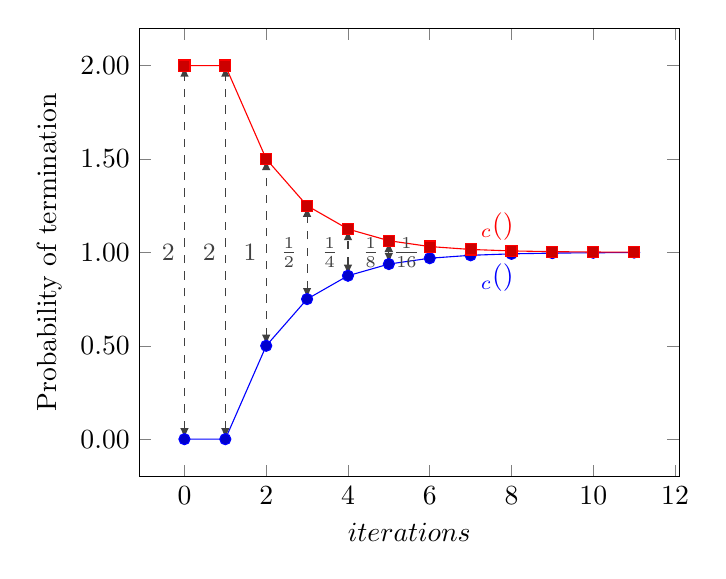
\begin{tikzpicture}
\begin{axis}[%[ybar] 
    xlabel={$iterations$},
    ylabel={Probability of termination},
    y tick label style={/pgf/number format/.cd,fixed,fixed zerofill,precision=2},
]
    \addplot table[header=false,col sep=&,row sep=\\,y expr={\thisrowno{1}}] {
        0 & 0\\
        1 & 0\\
        2 & 1 - 1/2^1\\
        3 & 1 - 1/2^2\\
        4 & 1 - 1/2^3\\
        5 & 1 - 1/2^4\\
        6 & 1 - 1/2^5\\
        7 & 1 - 1/2^6\\
        8 & 1 - 1/2^7\\
        9 & 1 - 1/2^8\\
        10& 1 - 1/2^9\\
        11& 1 - 1/2^10\\
        %12& 1 - 1/2^11\\
        %13& 1 - 1/2^12\\
        %14& 1 - 1/2^13\\
        %15& 1 - 1/2^14\\
    } node[below,pos=0.7] {$\lfun_c(\ufzero)$};

    \addplot table[header=false,col sep=&,row sep=\\,y expr={\thisrowno{1}}] {
        0 & 2\\
        1 & 2\\
        2 & 2/2^1 + 1 - 1/2^1 \\
        3 & 2/2^2  + 1 - 1/2^2 \\
        4 & 2/2^3  + 1 - 1/2^3 \\
        5 & 2/2^4  + 1 - 1/2^4 \\
        6 & 2/2^5  + 1 - 1/2^5 \\
        7 & 2/2^6  + 1 - 1/2^6 \\
        8 & 2/2^7  + 1 - 1/2^7 \\
        9 & 2/2^8  + 1 - 1/2^8 \\
        10& 2/2^9  + 1 - 1/2^9 \\
        11& 2/2^10 + 1 - 1/2^10\\
        %12& 2/2^11 + 1 - 1/2^11\\
        %13& 2/2^12 + 1 - 1/2^12\\
        %14& 2/2^13 + 1 - 1/2^13\\
        %15& 2/2^14 + 1 - 1/2^14\\
    } node[above,pos=0.7] {$\lfun_c(\ufone)$};

    % \draw (axis cs:1,0) -- node[left]{Text} (axis cs:1,2);
    \draw[latex-latex, darkgray, dashed] (axis cs:0,0) -- node[left]{\small 2} (axis cs:0,2);
    \draw[latex-latex, darkgray, dashed] (axis cs:1,0) -- node[left]{\small 2} (axis cs:1,2);
    \draw[latex-latex, darkgray, dashed] (axis cs:2, 1 - 1/2^1) -- node[left]{\small 1} (axis cs:2, 2/2^1 + 1 - 1/2^1);
    \draw[latex-latex, darkgray, dashed] (axis cs:3, 1 - 1/2^2) -- node[left]{\small $\frac{1}{2}$} (axis cs:3, 2/2^2 + 1 - 1/2^2);
    \draw[latex-latex, darkgray, dashed] (axis cs:4, 1 - 1/2^3) -- node[left]{\small $\frac{1}{4}$} (axis cs:4, 2/2^3 + 1 - 1/2^3);
    \draw[latex-latex, darkgray, dashed] (axis cs:5, 1 - 1/2^4) -- node[left]{\small $\frac{1}{8}$} (axis cs:5, 2/2^4 + 1 - 1/2^4);
    \draw[latex-latex, darkgray, dashed] (axis cs:6, 1 - 1/2^5) -- node[left]{\small $\frac{1}{16}$} (axis cs:6, 2/2^5 + 1 - 1/2^5);
    %\draw[latex-latex, darkgray, dashed] (axis cs:7, 1 - 1/2^6) -- (axis cs:7, 2/2^6 + 1 - 1/2^6);
    % \addplot[mark=*, red, dashed] table[header=false,col sep=&,row sep=\\,y expr={\thisrowno{1}}] {
%        0 & 0\\
%        0 & 2\\
%    };
  \end{axis}
\end{tikzpicture}
    \end{center}
    \caption{Termination probability over iterations from bottom and top for coin flip.}
    \label{fig:coin_t_prob_iteration}
\end{figure}
%
As shown in the diagram, along with the increasing iterations, $\left(\lfun_c\right)^n (\ufzero)$ increases towards 1 from the initial 0, while $\left(\lfun_c\right)^n (\ufone)$ decreases towards 1 from the initial 2. Their differences, marked with dashed lines, are becoming smaller and smaller.
From this example, we observe that there is one unique fixed point where the least fixed point and the greatest fixed point are the same. The precondition for this uniqueness is their iteration differences converging to 0. If this is the case, in order to reason about a probabilistic loop, we just need to find out a fixed point and prove it. Then the fixed point is the semantics of the loop. Actually, we do not need to compute it by iterations. 

This example motivates us to give a semantics to probabilistic loops as follows.
First, we need to prove the loop function is continuous. Then if the differences of iterations from top and bottom converges to 0, there is a unique fixed point. Otherwise, we use the Kleene fixed-point Theorem~\ref{thm:kleene_fixed_point_theorem} to compute the least fixed point and the greatest fixed point by iterations.

\subsection{Fixed point theorems}
We define the function $\iter$ below recursively for iterations $(\lfun_P^b)^n(X)$, and the function $\iterdiff$ for the differences between iterations from top and bottom.
\begin{definition}[Iteration and iteration difference]
    \isalink{https://github.com/RandallYe/probabilistic_programming_utp/blob/336ff3c17af12fd71446a50244ff04966bfa71e8/probability/probabilistic_relations/utp_prob_rel_lattice.thy\#L405}
    \begin{align*}
        &\iter\left(n, b, P, X\right) \defs \left(\IF n = 0 \THEN X \ELSE \lfunbp\left(\iter\left(n-1, b, P, X\right)\right)\right)\tag*{(iteration)} \label{def:iter}\\
        &\lfundiff(b,P,X) \defs~\pcchoice{b}{\left(\pseq{P}{X}\right)}{\clz \ufzero} \\%\tag*{(loop function bottom)} \label{def:lfundiff} \\ 
        % &\iterdiff\left(n, b, P, X\right) \defs \left(\IF n = 0 \THEN X \ELSE \left(\pcchoice{b}{\left(\pseq{P}{\iterdiff\left(n-1, b, P, X\right)}\right)}{\ufzero}\right)\right)\tag*{(iteration difference)} \label{def:iterdiff}
        &\iterdiff\left(n, b, P, X\right) \defs \left(\IF n = 0 \THEN X \ELSE \lfundiff\left(b, P, \iterdiff\left(n-1, b, P, X\right)\right)\right)\tag*{(iteration difference)} \label{def:iterdiff}
    \end{align*}
\end{definition}
The $\lfundiff$ is similar to $\lfun$ in Definition~\ref{def:lfun} except that if the condition $b$ does not hold, it is $\ufzero$ instead of $\pskip$ in $\lfun$.

We show that the iteration from bottom is an ascending chain and the iteration from top is a descending chain if $P$ is a distribution.
\begin{thm}%[Iteration from bottom is an ascending chain]
    \label{thm:iter_bot_ascending}
   $\isfinaldist\left(\prrvfunsym{P}\right) \implies \incseq\left(\lambda n @ \iter\left(n, b, P, \ufzero\right)\right)$ 
   \isalink{https://github.com/RandallYe/probabilistic_programming_utp/blob/336ff3c17af12fd71446a50244ff04966bfa71e8/probability/probabilistic_relations/utp_prob_rel_lattice_laws.thy\#L4291}
\end{thm}

\begin{thm}%[Iteration from top is a descending chain]
    \label{thm:iter_top_descending}
   $\isfinaldist\left(\prrvfunsym{P}\right) \implies \decseq\left(\lambda n @ \iter\left(n, b, P, \ufone\right)\right)$ 
   \isalink{https://github.com/RandallYe/probabilistic_programming_utp/blob/336ff3c17af12fd71446a50244ff04966bfa71e8/probability/probabilistic_relations/utp_prob_rel_lattice_laws.thy\#L4331}
\end{thm}

For an ascending or descending chain $f$, we define $\finstatesasc$ and $\finstatesdes$ to denote there are only finite states to have their suprema or infima different from their initial values $f(0)$.
\begin{definition}[Finite states]
    \label{def:finstates}
    We fix $f: \nat \fun [S]\prhfun$, then define
    \isalink{https://github.com/RandallYe/probabilistic_programming_utp/blob/5558d7350b75fd5c1914dd8618d95bfad9e2f789/probability/probabilistic_relations/utp_prob_rel_lattice.thy\#L395}
    \begin{align*}
        \finstatesasc(f) & \defs \finite\left(\left\{s : S \mid \left(\left(\thnsup n @ f(n,s)\right) > f(0,s) \right)\right\}\right) \\
        \finstatesdes(f) & \defs \finite\left(\left\{s : S \mid \left(\left(\thninf n @ f(n,s)\right) < f(0,s) \right)\right\}\right)
    \end{align*}
\end{definition}
The intuition behind the definitions of $\finstatesasc$ and $\finstatesdes$ is that if an ascending or descending chain $f$ has its supremum or infimum not equal to $f(0)$ for a particular state $s$, then there exists a $m:\nat$ such that for any $\varepsilon:\real > 0$, $\left(\thnsup n @ f(n,s) - f(m,s) < \varepsilon\right)$ or $\left(f(m,s) - \thninf n @ f(n,s)  < \varepsilon\right)$. 
%$f(m, s) = f(0, s)$ and $f(m+1, s) > f(m, s)$ or $f(m+1, s) < f(m, s)$.
%
% \begin{definition}[Finite final states]
% %   $finite(P) = \finite\left(\left\{s : S | P(s)\right\}\right)$
% %   $fin\_states(P) = finite\left(\lambda s : S \times S @ \exists n @ \iter\left(n, b, P, \ufzero\right)\right)$
%     \begin{align*}
%         \finstates(f) & \defs \finite\left(\left\{s : S | \left(\left(\thnsup n @ f(n,s)\right) > f(0,s) \right)\right\}\right) \\
%         \finstatesnzero(b, P) & \defs \finite\left(\left\{s : S \times S | \left(\exists n @ \iter\left(n, b, P, \ufzero\right) s \neq 0 \right)\right\}\right) \\
%         \finstatesnone(b, P) & \defs \finite\left(\left\{s : S \times S | \left(\exists n @ \iter\left(n, b, P, \ufone\right) s \neq 1 \right)\right\}\right)
%     \end{align*}
% \end{definition}

We show that if $f$ is an ascending chain and also $\finstatesasc(f)$, then there exists a $N:\nat$ such that for any $n\geq N$, $f(n,s)$ is close to its supremum in a given distance $\varepsilon : \real > 0$ for any $s$. 
\begin{thm}
    \label{thm:incseq_limit_is_lub_all}
    We fix $f:\nat \fun [S_1,S_2]\prfun$, then 
    \isalink{https://github.com/RandallYe/probabilistic_programming_utp/blob/5558d7350b75fd5c1914dd8618d95bfad9e2f789/probability/probabilistic_relations/utp_prob_rel_lattice_laws.thy\#L3487}
    \begin{align*}
        & \incseq(f) \land \finstatesasc(f) \implies \forall \varepsilon:\real > 0 \bullet \exists N:\nat \bullet \forall n \geq N \bullet \forall s \bullet \left(\thnsup m @ f(m, s)\right) - f(n,s) < \varepsilon %\\
%        & \decseq(f) \land \finstatesdes(f) \implies \forall \varepsilon:\real > 0 \bullet \exists N:\nat \bullet \forall n \geq N \bullet \forall s \bullet f(n,s) - \left(\thnsup m @ f(m, s)\right) < \varepsilon
    \end{align*}
\end{thm}

\begin{figure}[!ht]
    \begin{center}
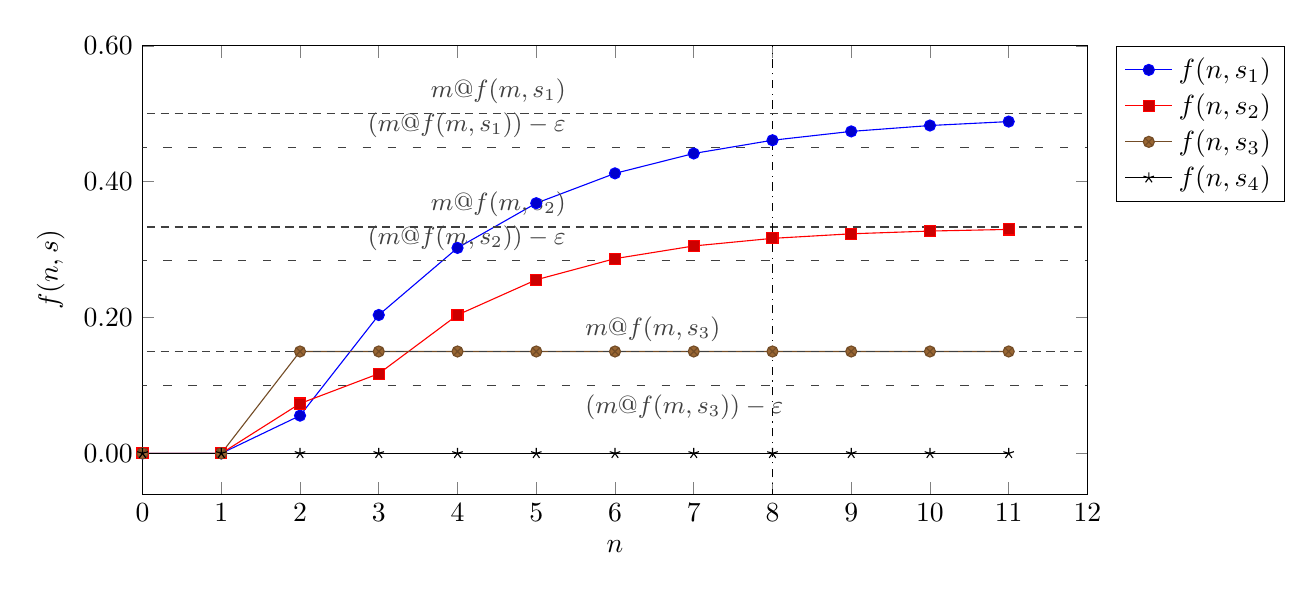
\begin{tikzpicture}
\begin{axis}[%[ybar] 
    xlabel={$n$},
    xmin=0,
    xmax=12,
    x=1.0cm,
    ymax=0.6,
    ylabel={$f(n,s)$},
    y tick label style={/pgf/number format/.cd,fixed,fixed zerofill,precision=2},
    legend pos=outer north east,
]
    \addplot table[header=false,col sep=&,row sep=\\,y expr={\thisrowno{1}}] {
        0 & 0\\
        1 & 0\\
        2 & 1/2 - (2/3)^2\\
        3 & 1/2 - (2/3)^3\\
        4 & 1/2 - (2/3)^4\\
        5 & 1/2 - (2/3)^5\\
        6 & 1/2 - (2/3)^6\\
        7 & 1/2 - (2/3)^7\\
        8 & 1/2 - (2/3)^8\\
        9 & 1/2 - (2/3)^9\\
        10& 1/2 - (2/3)^10\\
        11& 1/2 - (2/3)^11\\
        %12& 1 - 1/2^11\\
        %13& 1 - 1/2^12\\
        %14& 1 - 1/2^13\\
        %15& 1 - 1/2^14\\
    } node[below right,pos=0.7] {};
    \addlegendentry{$f(n,s_1)$};

    \addplot table[header=false,col sep=&,row sep=\\,y expr={\thisrowno{1}}] {
        0 & 0\\
        1 & 0\\
        2 & 1/3 - (3/5)^2 + 0.1\\
        3 & 1/3 - (3/5)^3\\
        4 & 1/3 - (3/5)^4\\
        5 & 1/3 - (3/5)^5\\
        6 & 1/3 - (3/5)^6\\
        7 & 1/3 - (3/5)^7\\
        8 & 1/3 - (3/5)^8\\
        9 & 1/3 - (3/5)^9\\
        10& 1/3 - (3/5)^10\\
        11& 1/3 - (3/5)^11\\
        %12& 1 - 1/2^11\\
        %13& 1 - 1/2^12\\
        %14& 1 - 1/2^13\\
        %15& 1 - 1/2^14\\
    } node[below right,pos=0.7] {};
    % \draw (axis cs:1,0) -- node[left]{Text} (axis cs:1,2);
    \addlegendentry{$f(n,s_2)$};

    \addplot table[header=false,col sep=&,row sep=\\,y expr={\thisrowno{1}}] {
        0 & 0\\
        1 & 0\\
        2 & 0.15\\
        3 & 0.15\\
        4 & 0.15\\
        5 & 0.15\\
        6 & 0.15\\
        7 & 0.15\\
        8 & 0.15\\
        9 & 0.15\\
        10& 0.15\\
        11& 0.15\\
        %12& 1 - 1/2^11\\
        %13& 1 - 1/2^12\\
        %14& 1 - 1/2^13\\
        %15& 1 - 1/2^14\\
    } node[below right,pos=0.7] {};
    \addlegendentry{$f(n,s_3)$};

    \addplot table[header=false,col sep=&,row sep=\\,y expr={\thisrowno{1}}] {
        0 & 0\\
        1 & 0\\
        2 & 0\\
        3 & 0\\
        4 & 0\\
        5 & 0\\
        6 & 0\\
        7 & 0\\
        8 & 0\\
        9 & 0\\
        10& 0\\
        11& 0\\
        %12& 1 - 1/2^11\\
        %13& 1 - 1/2^12\\
        %14& 1 - 1/2^13\\
        %15& 1 - 1/2^14\\
    } node[above right,pos=0.7] {};
    \addlegendentry{$f(n,s_4)$};

    % \draw[darkgray] (axis cs:-1,0.5) -- (axis cs:12,0.5);
    % \node[black,right] at (axis cs:12,0.5){\small $\thnsup m @ f(m,s_1)$};
    % %\draw[darkgray,dashed] (axis cs:-1,0.45) -- node[above right]{\small $\left(\thnsup m @ f(m,s_1)\right) - \varepsilon$} (axis cs:12,0.45);
    % \draw[darkgray,dashed] (axis cs:-1,0.45) -- (axis cs:12,0.45);
    % \node[black,right] at (axis cs:12,0.45){\small $\left(\thnsup m @ f(m,s_1)\right) - \varepsilon$};
    \draw[darkgray,densely dashed] (axis cs:-1,0.5) -- node[above left]{\small $\thnsup m @ f(m,s_1)$} (axis cs:12,0.5);
    \draw[darkgray,loosely dashed] (axis cs:-1,0.45) -- node[above left]{\small $\left(\thnsup m @ f(m,s_1)\right) - \varepsilon$} (axis cs:12,0.45);

    \draw[darkgray,densely dashed] (axis cs:-1,1/3) -- node[above left]{\small $\thnsup m @ f(m,s_2)$} (axis cs:12,1/3);
    \draw[darkgray,loosely dashed] (axis cs:-1,1/3-0.05) -- node[above left]{\small $\left(\thnsup m @ f(m,s_2)\right) - \varepsilon$} (axis cs:12,1/3-0.05);

    \draw[darkgray,densely dashed] (axis cs:-1,0.15) -- node[above right]{\small $\thnsup m @ f(m,s_3)$} (axis cs:12,0.15);
    \draw[darkgray,loosely dashed] (axis cs:-1,0.1) -- node[below right]{\small $\left(\thnsup m @ f(m,s_3)\right) - \varepsilon$} (axis cs:12,0.1);

    \draw[black,dashdotted] (axis cs:8,-1) -- node[above left]{\small $N$} (axis cs:8,0.6);
  \end{axis}
\end{tikzpicture}
    \end{center}
    \caption{Illustration of limits of a increasing chain for various states.}
    \label{fig:finitestateasc}
\end{figure}
%

This is explained and illustrated in Fig.~\ref{fig:finitestateasc} where $f$ is a monotonic function, such as $\left(\lambda n @ \iter\left(n, b, P, \ufzero\right)\right)$, whose domain is a complete lattice, and so its limit exists and is the supremum ($\thnsup n@ f(n,s_i)$) of the increasing chain of this function for a particular state $s_i$. In this diagram, we show there are four states (four combinations of the product states $(s,s')$, indeed) in the observation space, denoted as $s_1$,$s_2$,$s_3$, and $s_4$. We draw the function $f$ of the four states for $n$ up to 11, as shown in the diagram as $f(n,s_1)$, $f(n, s_2)$, $f(n, s_3)$, and $f(n, s_4)$. The function for each state has a corresponding supremum, such as $\thnsup n @ f(n,s_1)$ for $s_1$, and a densely dashed line denotes the supremum. We also consider a real number $\varepsilon > 0$ and so Epsilon regions are formed between the densely dashed lines (the supremum) and the loosely dashed line ($\left(\thnsup n @ f(n,s_i)\right) - \varepsilon$). The theorem above shows there is always a $N$ for all $m \geq N$ such that the closeness of $f(m,s_i)$ to its supremum ($\thnsup n@ f(n,s_i)$) is less than $\varepsilon$ for any $s_i$. Because the limit of $f(n,s_i)$ is $\left(\thnsup n @ f(n,s_i)\right)$, there always exists a $N_i$ to satisfy this closeness. For constant zero functions such as $f(n,s_4)$, $N_i$ is just 0. According to the assumption of finiteness, there are finite states to have their $N_i$ larger than 0, the states $\{s_1, s_2, s_3\}$, in this example, whose $N_i$ are 8, 6, and 2 respectively. We can choose $N$ as the maximum number from this $N_i$ set and it is 8 (illustrated as a dotted dash line at $x=8$) here. Now for all $n \geq N$ and any state $s$, the function $f(n,s)$ is close to its supremum within the given $\varepsilon$. This theorem is necessary to prove Theorem~\ref{thm:lfun_limit_as_supremum} below and eventually the continuity theorem~\ref{thm:continuity_lfun_bot}.

A descending chain $f$ satisfies the similar theorem below.
\begin{thm}
    \label{thm:decseq_limit_is_glb_all}
    We fix $f:\nat \fun [S_1,S_2]\prfun$, then 
    \isalink{https://github.com/RandallYe/probabilistic_programming_utp/blob/5558d7350b75fd5c1914dd8618d95bfad9e2f789/probability/probabilistic_relations/utp_prob_rel_lattice_laws.thy\#L3811}
    \begin{align*}
%        & \incseq(f) \land \finstatesasc(f) \implies \forall \varepsilon:\real > 0 \bullet \exists N:\nat \bullet \forall n \geq N \bullet \forall s \bullet \left(\thnsup m @ f(m, s)\right) - f(n,s) < \varepsilon \\
        & \decseq(f) \land \finstatesdes(f) \implies \forall \varepsilon:\real > 0 \bullet \exists N:\nat \bullet \forall n \geq N \bullet \forall s \bullet f(n,s) - \left(\thnsup m @ f(m, s)\right) < \varepsilon
    \end{align*}
\end{thm}

%\begin{thm}[Limit as supremum]
%    We fix $f:\nat \fun [S_1,S_2]\prfun$, 
%    \begin{align*}
%    & incseq(f) \implies \forall s @ \left(\lambda n:\nat @ f(n, s)\right) \tendsto \left({\thnsup n @ f\left(n, s\right)} \right)
%    \end{align*}
%\end{thm}

From Theorems~\ref{thm:iter_bot_ascending} and~\ref{thm:incseq_limit_is_lub_all}, we prove the following theorem stating that for any state $s$ the limit of the application of $\lfun$ to $\iter$ is the application of $\lfun$ to the supremum of iterations.
\begin{thm}[Limit as supremum]
    \label{thm:lfun_limit_as_supremum}
    \isalink{https://github.com/RandallYe/probabilistic_programming_utp/blob/5558d7350b75fd5c1914dd8618d95bfad9e2f789/probability/probabilistic_relations/utp_prob_rel_lattice_laws.thy\#L4359}
    \begin{align*}
        \begin{array}[]{l}
        \left(
            \isfinaldist\left(\prrvfunsym{P}\right) \land 
            \finstatesasc\left(\lambda n @ \iter\left(n, b, P, \ufzero\right) \right) 
        \right) \implies \\
        \forall s @ \left(\lambda n:\nat @ \lfunbp\left({\iter\left(n, b, P, \ufzero\right)}\right)(s)\right) \tendsto \left(\lfunbp\left({\thnsup n @ \iter\left(n, b, P, \ufzero\right)}\right)(s)\right)
        \end{array}
    \end{align*}
\end{thm}

From Theorems~\ref{thm:iter_top_descending} and~\ref{thm:decseq_limit_is_glb_all}, we prove the following similar theorem stating that for any state $s$ the limit of the application of $\lfun$ to $\iter$ is the application of $\lfun$ to the infimum of iterations.
\begin{thm}[Limit as infimum]
    \label{thm:lfun_limit_as_infimum}
    \isalink{https://github.com/RandallYe/probabilistic_programming_utp/blob/5558d7350b75fd5c1914dd8618d95bfad9e2f789/probability/probabilistic_relations/utp_prob_rel_lattice_laws.thy\#L4636}
    \begin{align*}
        \begin{array}[]{l}
        \left(
            \isfinaldist\left(\prrvfunsym{P}\right) \land 
            \finstatesdes\left(\lambda n @ \iter\left(n, b, P, \ufone\right) \right) 
        \right) \implies \\ 
        \forall s @ \left(\lambda n:\nat @ \lfunbp\left({\iter\left(n, b, P, \ufone\right)}\right)(s)\right) \tendsto \left(\lfunbp\left({\thninf n @ \iter\left(n, b, P, \ufone\right)}\right)(s)\right)
        \end{array}
    \end{align*}
\end{thm}

Continuity of $\lfun$ for iterations from bottom and top is derived from Theorems~\ref{thm:lfun_limit_as_supremum} and~\ref{thm:lfun_limit_as_infimum} and presented below.
\begin{thm}[Continuity - iteration from bottom]
    \label{thm:continuity_lfun_bot}
    \isalink{https://github.com/RandallYe/probabilistic_programming_utp/blob/5558d7350b75fd5c1914dd8618d95bfad9e2f789/probability/probabilistic_relations/utp_prob_rel_lattice_laws.thy\#L4604}
    \begin{align*}
        \begin{array}[]{l}
        \left(
        %\begin{array}[]{l}
            \isfinaldist\left(\prrvfunsym{P}\right) \land 
            \finstatesasc\left(\lambda n @ \iter\left(n, b, P, \ufzero\right) \right) 
        %\end{array}
        \right) 
        \implies \lfunbp{\left(\thnsup n @ \iter\left(n, b, P, \ufzero\right)\right)} = \left(\thnsup n @ \iter\left(n, b, P, \ufzero\right)\right)
        \end{array}
    \end{align*}
\end{thm}

\begin{thm}[Continuity - iteration from top]
    \label{thm:continuity_lfun_top}
    \isalink{https://github.com/RandallYe/probabilistic_programming_utp/blob/5558d7350b75fd5c1914dd8618d95bfad9e2f789/probability/probabilistic_relations/utp_prob_rel_lattice_laws.thy\#L4861}
    \begin{align*}
        \begin{array}[]{l}
        \left(
        %\begin{array}[]{l}
            \isfinaldist\left(\prrvfunsym{P}\right) \land 
            \finstatesdes\left(\lambda n @ \iter\left(n, b, P, \ufone\right) \right) 
        %\end{array}
        \right) 
        \implies \lfunbp{\left(\thninf n @ \iter\left(n, b, P, \ufone\right)\right)} = \left(\thninf n @ \iter\left(n, b, P, \ufone\right)\right)
        \end{array}
    \end{align*}
\end{thm}

%The poset $\left([S]\urexpr, \leq\right)$ is a directed-complete partial order (dcpo) because $\left([S]\urexpr, \leq\right)$ is a complete lattice according to Theorem~\ref{thm:ureal_func_complete} and a complete lattice is directed-complete.
The Kleene fixed-point theorem~\ref{thm:kleene_fixed_point_theorem} states the least (or greatest) fixed point of a continuous function $\lfun$ is the supremum (or infimum) of the ascending (or descending) chain of the function. This is just the semantics of while loops. 
\begin{thm}[Least fixed point by construction]
    \label{thm:rec_least_fixed_point}
    \isalink{https://github.com/RandallYe/probabilistic_programming_utp/blob/5558d7350b75fd5c1914dd8618d95bfad9e2f789/probability/probabilistic_relations/utp_prob_rel_lattice_laws.thy\#L4908}
    \begin{align*}
        \begin{array}[]{l}
        \left(
        %\begin{array}[]{l}
            \isfinaldist\left(\prrvfunsym{P}\right) \land 
            \finstatesasc\left(\lambda n @ \iter\left(n, b, P, \ufzero\right) \right) 
            % \finite\left(\left\{s : S \times S | \exists n @ \iter\left(n, b, P, \ufzero\right) s \neq 0 \right\}\right)
        %\end{array}
        \right)  
        \implies \pwhile{b}{P} = \left(\thnsup n @ \iter\left(n, b, P, \ufzero\right)\right)
        \end{array}
    \end{align*}
\end{thm}

\begin{thm}[Greatest fixed point by construction]
    \label{thm:rec_great_fixed_point}
    \isalink{https://github.com/RandallYe/probabilistic_programming_utp/blob/5558d7350b75fd5c1914dd8618d95bfad9e2f789/probability/probabilistic_relations/utp_prob_rel_lattice_laws.thy\#L4918}
    \begin{align*}
        \begin{array}[]{l}
        \left(
        %\begin{array}[]{l}
            \isfinaldist\left(\prrvfunsym{P}\right) \land
            \finstatesdes\left(\lambda n @ \iter\left(n, b, P, \ufone\right) \right) 
        %\end{array}
        \right)  
        \implies \pwhiletop{b}{P} =\left(\thninf n @ \iter\left(n, b, P, \ufone\right)\right)
        \end{array}
    \end{align*}
\end{thm}
There are several benefits to have the semantics of probabilistic loops constructed by iterations, as shown in Theorems~\ref{thm:rec_least_fixed_point} and~\ref{thm:rec_great_fixed_point}. Essentially, the theorems give the semantics to probabilistic loops theoretically. In practice, they also enable us to compute the semantics by approximation or iterations, for example, in model checking.
Another benefit is to facilitate the proof of the unique fixed point theorem as follows.

\begin{thm}[Unique fixed point] \label{thm:rec_unique}
    \isalink{https://github.com/RandallYe/probabilistic_programming_utp/blob/5558d7350b75fd5c1914dd8618d95bfad9e2f789/probability/probabilistic_relations/utp_prob_rel_lattice_laws.thy\#L5298}
    \begin{align*}
        & %\left(
        \begin{array}[]{l}
            \isfinaldist\left(\prrvfunsym{P}\right) \land 
            \finstatesasc\left(\lambda n @ \iter\left(n, b, P, \ufzero\right) \right) \land 
            \forall s @ \left(\lambda n @ \prrvfunsym{\iterdiff\left(n, b, P, \ufone\right)}(s)\right) \tendsto 0 \land 
            \lfunbp\left(fp\right) = fp
        \end{array} %\right) 
        \\
        & \implies \left(\pwhile{b}{P} = fp\right) \land \left(\pwhiletop{b}{P} = fp\right) 
    \end{align*}
\end{thm}
There are four assumptions in the theorem. The third one corresponds to the differences between iterations from top and bottom, illustrated as dashed lines in Fig.~\ref{fig:coin_t_prob_iteration}. If for any state $s$, the difference tends to 0, then the least fixed point by Theorem~\ref{thm:rec_least_fixed_point} and the greatest fixed point by Theorem~\ref{thm:rec_great_fixed_point} coincide. The fourth assumption states $fp$ is a fixed point of $\lfun$. The conclusion states that both the least fixed point and the greatest fixed point are just $fp$.  
With this theorem, the proof obligation for reasoning about loops is largely simplified just to establish these assumptions.

%% The Case Studies
\subsection{Attacking Weight-based Watermarks}
\label{sec:eval_weight}
% \noindent\textit{7.2.1$\quad$Uchida et al.}\\
\noindent\textbf{(1) Uchida et al.}
% This method utilizes a watermark-related regularization term to embed owner-specific information into the certain weights of a layer of the target model, 
Uchida et al.\cite{uchida2017embedding} introduce one of the earliest white-box schemes which embed the model watermark into the convolutional weights of the target model. 
% As we mentioned in Section \ref{sec: white-box wm}
To extract the model watermark, the scheme first averages the convolutional weights $w \in \mathbb{R}^{N_{l-1}\times N_l \times w \times h}$ of the watermark-related layer through first dimension and flattens the weight to $\hat w \in \mathbb{R}^{(N_l \cdot w \cdot h)}$. Then, a binary string $s'$ is obtained from $\hat w$ through a pre-defined linear matrix $A$ and a threshold function $T_h$ at 0, i.e.,
%%%%%%%%%%%%%%%%%%%%% begin eq uchida %%%%%%%%%%%%%%%%%%%%%
% \begin{equation}\label{eq:uchida}
$
s' = T_h(X \cdot \hat w),
$
% \end{equation}
%%%%%%%%%%%%%%%%%%%%% end eq uchida %%%%%%%%%%%%%%%%%%%%%
which is matched with the owner-specific message $s$ in terms of BER for validation.
% where $T_h$ is a hard threshold function which outputs $1$ when the input is positive and $0$ otherwise. Finally, the extracted binary string $s'$ is matched with the owner-specific message $s$ in terms of BER to assert the model ownership.

\noindent$\bullet$\textbf{ Discussion.}
% As the linear transformation matrix in \ref{eq:uchida} is predefined before the watermark embedding procedure,  As the extraction process of Uchida et al. only consists of a mask matrix and a linear transformation matrix, \mytodo{the element-level representations of watermark-related parameters play a crucial role to the final extracted binary string. (please be more pointed at its own weakness)}
Although this approach is previously shown to be vulnerable to overwriting, known attacks however require the specific prior knowledge of the watermark algorithm as well as a domain dataset, both of which are usually impractical. Our attack reveals the insecurity of this algorithm by directly modifying the structure of the target model while leaving the utility intact. Specifically, the dimension of $\hat w$ is increased once the adversary injects dummy neurons into watermark-related layers. As a result, during the extraction procedure of $s_i'$ from the victim model, the second dimension of pre-defined linear transformation matrix $X$ is unmatched to the dimension of expanded $\hat w$ any longer.

%%%%%%%%%%%%% BEGIN OF ls fig
%\begin{figure}[t]
%\begin{center}
%\includegraphics[width=0.45\textwidth]{img/ber_p_uchida_dn.pdf}
%\caption{BER of WRN watermarked by \cite{uchida2017embedding} after an $\alpha$ ratio of dummy neurons are injected by our attacks. The dashed horizontal lines reports the BER of an irrelevant model.}
%\label{fig:ber_p_uchida}
%\end{center}
%\vspace{-0.25in}
%\end{figure}
%%%%%%%%%%%%%% END OF ls fig

\noindent$\bullet$\textbf{ Evaluation Results.}
We run the code of \cite{code-uchida} they publicly released to reproduce a watermarked model of Wide Residual Network (WRN) trained on CIFAR10 dataset. We perform our removal attack to inject dummy neurons generated via different methods into each layer, which presents the same original utility with classification accuracy of $91.55\%$ while the verification procedure is inhibited if with no error handling mechanism. As Fig.\ref{fig:scaled_ber} shows that applying Max-First cannot restore the embedded watermark from structural obfuscated model by \textit{NeuronClique} and \textit{NeuronSplit}, as the BER is increased over $50\%$ once we add less than $5\%$ dummy neurons, indicating the innate vulnerability of this scheme.


% ########################################################################
\noindent\textbf{(2) RIGA.} Wang et al. \cite{wang2021riga} replace the linear transformation matrix in Uchida et al. with a learnable fully-connected neural network (FCN) to boost the encoding capacity of watermarking messages. That is, the intuition behind this watermark scheme is closely identical to Uchida et al. We present the full details in Appendix \ref{sec:app:eval} and report the results in Fig.\ref{fig:scaled_ber}.
% \noindent\textbf{Protection Mechanism.}
% Wang et al. \cite{wang2021riga} enhance the covertness and robustness of prior white-box watermarking methods against watermark detection and removal attacks based on adversarial training and more sophisticated transformation function. They train a watermark detector to serve as a discriminator to encourage the distribution of watermark-related weights to be similar to that of unwatermarked models. Meanwhile, they replace the watermark extractor, which is previously implemented with a predefined linear transformation \cite{uchida2017embedding}, with a learnable fully-connected neural network (FCN), for boosting the encoding capacity of watermarking messages. Similar to Uchida et al.\cite{uchida2017embedding}, the watermark-related weights are first selected from the target model and then projected to a binary string $s'$ via the FCN-based extractor during the ownership verification procedure.



% \noindent\textbf{Discussion.}
% Simply replacing the linear transformation matrix in Uchida et al. \cite{uchida2017embedding} to a learnable extractor can not completely eliminate the removal threats from our attack based on model structural obfuscation. As a result, RIGA has the similar vulnerability of \cite{uchida2017embedding} as their watermark extraction procedures only differ into the type of extractor, which is also inexecutable due to the incompatible input dimension of the trained extractor for RIGA.


% \noindent\textbf{Evaluation Results.}
% We follow their evaluation settings to watermark Inception-V3 trained on CelebA, which achieves $95.90\%$ accuracy and $0\%$ BER \cite{code-riga}. We employ the default setups that the watermark is embedded into the third convolutional layer of the target model and the extractor is a multiple layer perceptron with one hidden layer. With our attack framework, we successfully inhibit the ownership verification of RIGA without any loss to the utility of victim model. Even applying the error-handling mechanisms, the BER of extracted message is increased to an unacceptable level. For example, when we utilize Max-First error-handling to obtain the embedded watermark, the BER is increased to $23.75\%$ when we inject the dummy neurons generated via \textit{NeuronSplit}.

% ########################################################################
\noindent\textbf{(3) IPR-GAN.}
To extend the watermarking primitive to generative adversarial networks (GANs) \cite{goodfellow2014gan}, Ong et al. present the first model watermark framework which first invokes black-box verification to collect some evidence from the suspect model via remote queries, and then utilizes the white-box verification for further extracting the watermark from the specific weights of suspicious model through the law enforcement. Different from \cite{uchida2017embedding}, Ong et al. embed the identification information into the scale parameters $\gamma$ of the normalization layers, rather than the convolutional weights. Correspondingly, the transformation function used in watermark verification stage consists of only a hard threshold function $T_h$, which actually extracts the signs of $\gamma$ in selected normalization layers as a binary string, i.e., 
%%%%%%%%%%%%%%%%%%%%% begin eq iprgan %%%%%%%%%%%%%%%%%%%%%
% \begin{equation}\label{eq:iprgan}
$s' = T_h(\gamma).$
% \end{equation}
%%%%%%%%%%%%%%%%%%%%% end eq iprgan %%%%%%%%%%%%%%%%%%%%%

\noindent$\bullet$\textbf{ Discussion.}
We focus on the white-box part of the watermark method. Previous works have shown that the scale parameters $\gamma$ of normalization layers are more stable than the convolution weights against existing removal attacks and ambiguity attacks, as small perturbation to these watermark-related parameters would cause significant drops to the original model utility. However, the number of scale weights in the watermark-related layer can be increased once we inject a group of dummy neurons. As a result, the length of binary string $s'$ extracted by the transformation function $T_h$ in this watermarking scheme is incompatible with the length of the target watermark any longer.
%As a result, the extracted binary string in Equation \ref{eq:iprgan} can be arbitrarily modified. 
% The capacity of embedded information is constrained by the total number of channels in normalization layers.

\noindent$\bullet$\textbf{ Evaluation Results.}
We follow their evaluation setups to watermark DCGAN trained on the CUB200 dataset, which achieves $54.33$ in terms of FID and has $0\%$ BER \cite{code-iprgan}.
As the watermark verification procedure is blocked with our proposed removal attacks, we leverage the error-handling methods on the scale weights to measure the BER of the extracted signature, which only has at most $55.86\%$ matched bits to the pre-defined binary signature while the FID of the generator is perfectly preserved as $54.33$, as  Fig.\ref{fig:scaled_ber} shows.

% ########################################################################
\noindent\textbf{(4) Greedy.}
Liu et al. \cite{liu2021greedyresiduals} propose to greedily select fewer yet more important model weights called the \textit{greedy residuals}, which is more important to the normal model utility and hence improves the watermark robustness against previous attacks. Specifically, the method extracts the identity information by first applying the transformation function $A$ on the one-dimensional average pooling over the flattened parameters $\hat w$ in the chosen convolutional layers, and then greedily takes the largest absolute values in each row by a ratio of $\eta$ to build the residuals. Finally, the secret binary string can be extracted from the signs of residuals by hard threshold function $T_h$ after being averaged to a real-valued vector.
Formally, the extraction procedure can be written as
%%%%%%%%%%%%%%%%%%%%% begin eq greedy %%%%%%%%%%%%%%%%%%%%%
% \begin{equation}\label{eq:greedy}
$
s' = T_h(Avg(Greedy(Avg\_pool\_1D(\hat w)))).
$
% \end{equation}
%%%%%%%%%%%%%%%%%%%%% end eq greedy %%%%%%%%%%%%%%%%%%%%%

\noindent$\bullet$\textbf{ Discussion.}
Greedy Residuals utilize some important parameters for embedding, which are more stable than choosing all the convolution weights in the specific layer proved in their ablation evaluations. Moreover, this watermark scheme greedily select the larger absolute values in each row from the intermediate feature matrix to build the residuals with fixed number of values, the verification procedure is not inhibited with the injection of dummy neurons. However, as the average pooled feature matrix before residual construction is impacted by some arbitrary values introduced by the injected dummy neurons, the extracted watermark after our attack would be perturbed unexpectedly. 
% As Greedy Residuals is still executable on the obfuscated model, we do not report the results of error-handling the watermark extraction algorithm in Table \ref{tab:eval}.

\noindent$\bullet$\textbf{ Evaluation Results.}
We run the source codes of Greedy Residuals publicly released by the authors \cite{code-greedy} to reproduce a watermarked ResNet18 training on Caltech256 dataset with $55.05\%$ accuracy and $0\%$ BER. We embed the secret watermark on the parameters of the first convolution layer with $\eta = 0.5$. We prove that our removal attack can utterly destroy the model watermark embedded into the residual of fewer parameters, for example, leading to an increase in the BER to $57.57\%$ after injecting dummy neurons from \textit{NeuronClique} whereas the model utility remains unchanged.

% ########################################################################
% sparsity pattern 
\noindent\textbf{(5) Lottery.}
The Lottery Ticket Hypothesis (LTH) explores a new scheme for compressing the full model to reduce the training and inference costs. As the topological information of a found sparse sub-network (i.e., the winning ticket) is a valuable asset to the owners, Chen et al. propose a watermark framework to protect the IP of these sub-networks \cite{chen2021lottery}. Specifically, they take the structural property of the original model into account for ownership verification via embedding the watermark into the weight mask in several layers with highest similarity to enforce the sparsity masks to follow certain 0-1 pattern. The proposed lottery verification uses the QR code to increase the capacity of the watermark method. For watermark verification, this algorithm first selects a set of watermark-related weight masks $m$ and then averages the chosen masks to a 2-dimensional matrix, which is further transformed to a QR code via $Sign$ function, i.e., $s' = Sign(Avg(m))$ and can be validated via a QR scanner. 
%%%%%%%%%%%%%%%%%%%%% begin eq lottery %%%%%%%%%%%%%%%%%%%%%
% \begin{equation}\label{eq:lottery}
% s' = T_h(Avg(m))
% \end{equation}
%%%%%%%%%%%%%%%%%%%%% end eq lottery %%%%%%%%%%%%%%%%%%%%%

\noindent$\bullet$\textbf{ Discussion.}
While most existing watermark techniques explore the specific model weights or prediction to embed the secret watermark, the lottery verification leverages the sparse topological information (i.e., the weight masks) to protect the winning ticket by embedding a QR code which can be further decoded into the secret watermark. However, our attack directly obfuscates the topological information of the target model by injecting groups of dummy neurons with the corresponding weight masks, which enlarges the shape of extracted QR code from the weight mask of trained winning ticket unexpectedly. As this QR code without valid shape is not decodable, we leverage the error-handling mechanism to extract the embedded watermark for ownership verification, where remains a large distortion.

%%%%%%%%%%%%% BEGIN OF ls fig
\begin{figure}[t]
\begin{center}
\includegraphics[width=0.4\textwidth]{img/qrcode_dn.png}
\vspace{-0.2in}
\caption{The QR codes extracted from ResNet-20 watermarked by\cite{chen2021lottery} after an $\alpha$ ratio of dummy neurons are added.}
\label{fig:qrcode}
\end{center}
\vspace{-0.3in}
\end{figure}
%%%%%%%%%%%%%% END OF ls fig

\noindent$\bullet$\textbf{ Evaluation Results.}
We follow the evaluation settings in the original paper to watermark a ResNet20 training on CIFAR-100 dataset, which achieves $66.41\%$ accuracy and $0\%$ BER \cite{code-lottery}. Although the QR code has the ability to correct some errors which improves the robustness against existing attacks, the identity information decoding procedure from the extracted QR code is invalidated by adding only a few (e.g., $1\%$)  dummy neurons in the victim model as Fig.\ref{fig:qrcode} shows. Moreover, the original design of Lottery Ticket is inhibited (due to the unmatched size) when attackers insert the dummy neurons into the protected model, while it retains robust against structure obfuscation with our proposed error-handling mechanisms. In other words, Lottery Ticket would have better robustness against neural structural obfuscation than other schemes if the unmatched size of neural layers are properly addressed in its design. 

% ########################################################################
\subsection{Attacking Activation-based Watermarks}
\noindent\textbf{(1) DeepSigns.}
As a representative of activation-based white-box watermarking schemes, DeepSigns proposes to embed the model watermark into the probability density function (PDF) of the intermediate activation maps obtained in different layers on the white-box scenario. Specifically, DeepSigns adopts a Gaussian Mixture Model (GMM) as the prior probability to characterize the hidden representations, and considers the mean values of the PDF at specific layers to share the same role as the watermark-related weights in Uchida et al. \cite{uchida2017embedding}. Similar to the verification procedure of \cite{uchida2017embedding}, a transformation matrix $A$, randomly sampled in embedding procedure, projects the mean values of chosen intermediate features to a real-valued vector. With the final hard threshold function, the resulted binary string $s'$ is matched to the owner-specific watermark for claiming the model ownership. 

%%%%%%%%%%%%%%%%%%%%% begin eq greedy %%%%%%%%%%%%%%%%%%%%%
% \begin{equation}\label{eq:deepsign}
% s' = T_h(A \cdot \frac{1}{|D_T|}h^l(x_t; W^l_{in}))
% \end{equation}
%%%%%%%%%%%%%%%%%%%%% end eq greedy %%%%%%%%%%%%%%%%%%%%%

\noindent$\bullet$\textbf{ Discussion.}
% Most known attacks focus on carefully fine-tuning the victim model or utilizing some transformations to the trigger data to remove the inner watermarks embedded by DeepSigns \cite{chen2021refit}. As the element-level representations of the weights at specific layer (or channel) are closely related to the output feature maps, DeepSigns is almost as vulnerable as Uchida et al's under these attacks. However, these known attacks again involve impractical assumptions on the attacker's knowledge and sacrifice much of the normal model utility for fully removing the watermark. As a comparison, our attack utilize the local features of 
The notable difference between DeepSigns and \cite{uchida2017embedding} is where to embed the model watermark. 
However, as the hidden features utilized by DeepSigns are generated by the weights in the preceding layer, e.g., $a_i = W_i\cdot x+b_i$, the structural information of target model is closely related to the shape of output feature maps. 
For example, the shape of the watermark-related layer's output is expanded after injecting dummy neurons, which inhibits the ownership verification due to the incompatible dimension of the output activation maps and the pre-defined transform matrix.
As a result, DeepSigns is almost as vulnerable as \cite{uchida2017embedding} under our attack.


\noindent$\bullet$\textbf{ Evaluation Results.}
We run the source code of DeepSigns from \cite{code-deepsign} to watermark a wide residual network trained on CIFAR10. This watermarked WRN achieves $89.94\%$ accuracy and $0\%$ BER. With the error-handling method, it is shown that the ownership verification of the target model is completely confused by our removal attacks. For example, the BER is increased to $47.59\%$ with dummy neurons from \textit{NeuronSplit} while the original model functionality is intact.

\noindent\textbf{(2) IPR-IC.}
As previous watermarking schemes are mainly designed for image classification models, they are insufficient to IP protection for image captioning models and cause inevitable degradation to the image captioning performance. Therefore, Lim et al. \cite{lim2022ipcaption} embed a unique signature into Recurrent Neural Network (RNN) through hidden features. At the ownership verification stage, the mask matrix $M$ first selects the hidden memory state $h$ of given watermarking image in protected RNN model. Then, the hard threshold function transforms the chosen $h$ to a binary string $s'$, which can be formally written as
%%%%%%%%%%%%%%%%%%%%% begin eq lstm %%%%%%%%%%%%%%%%%%%%%
$
s' = T_h(h).$
%%%%%%%%%%%%%%%%%%%%% end eq lstm %%%%%%%%%%%%%%%%%%%%%

\noindent$\bullet$\textbf{ Discussion.}
Similar to DeepSigns \cite{darvish2019deepsigns} and IPR protection on GANs \cite{ong2021iprgan}, the topological information is closely related to the shape of hidden memory state. Although the protected image captioning model contains an RNN architecture, we can adopt our structural obfuscation method to expand the size of hidden state, e.g., with vanishing weights, to produce an equivalence of the original model with the same output.

\noindent$\bullet$\textbf{ Evaluation Results.}
We run the official implementation \cite{code-captioning} to reproduce a watermarked Resnet50-LSTM trained on COCO, which achieves $72.06$ BLEU-1 and has $0\%$ BER. With our proposed removal attacks, the signature extracted from the hidden memory state $h$ is not compatible to the size of the owner-specific binary message. We leverage error-handling mechanisms, e.g., Max-First to extract the identity message, which is perturbed with $56.95\%$ and $52.60\%$ BER for \textit{NeuronClique} and \textit{NeuronSplit}, while no loss is brought to the image captioning performance.

% \subsection {Passport-based}
% ########################################################################
\subsection{Attacking Passport-based Watermarks} %\label{section:DeepIPR}
\noindent\textbf{(1) DeepIPR.} 
DeepIPR is one of the earliest passport-based DNN ownership verification schemes \cite{fan2021deepip}. By inserting owner-specific passport layers during the watermark embedding procedure, DeepIPR is designed to claim the ownership not only based on the extracted signature from the specific model parameters but also on the model performance with the private passport layer. Consequently, this scheme shows high robustness to previous removal attacks and especially to the ambiguity attacks, which mainly forge counterfeit watermarks to cast doubts on the ownership verification.

In our evaluation, we focus on the following passport verification scheme in \cite{fan2021deepip}. This scheme generates two types of passport layers simultaneously by performing a multi-task learning, i.e., public passports for distribution and private passports for verification, both of which are actually based on normalization layers. Generally, DeepIPR leverages pre-defined digital passports $P=\{P_{\gamma}, P_{\beta}\}$ to obtain the scale and the bias parameters of the private passport, which are written as:
$
\gamma = Avg(W_c \odot P_{\gamma}), \beta =  Avg(W_c \odot P_{\beta}),
$
where $W_c$ is the filters of the precedent convolution layer, and $\odot$ denotes the convolution operation. DeepIPR adopts a similar watermark extraction process as \cite{uchida2017embedding}, where the transformation function $A$ converts the signs of the private $\gamma$ into a binary string to match the target signature.

\noindent$\bullet$\textbf{ Discussion.}
As the private $\gamma$ and $\beta$ are obtained from the preceding convolution weights, DeepIPR actually embeds the secret signature in the hidden output of the convolutional layer with the weights $W_c$ given the input $P_{\gamma}$ or $P_{\beta}$. Similar to the activation-based watermarking scheme, the unmatched extracted watermark can not be used to ownership verification due to the expanded shape of $W_c$.
% Specifically, the signs of private $\gamma$ can be modified directly by changing the signs of related convolution weights, \mytodo{which causes a significant damage to the watermark detection procedure and model performance with private layers (this sentence is ambiguous. Needs discussion).}
% However, because the joint training for different passport layers leads to different distribution of the feature maps before normalization, DeepIPR calculates statistic values of normalization layers on-the-fly by replacing the batch normalization to other normalization, which causes noticeable drops to the original performance



% %%%%% BEGIN sig TABLE
% % For accuracy, x/y stands for the model performance with public passport and private passport respectively.


% Table generated by Excel2LaTeX from sheet 'Sheet1'
\begin{table}[htbp]
  \centering
   \caption{Extracted signatures and the model accuracy when an $\alpha$ ratio of neurons are modified by our attack.}
    \begin{tabular}{clc}
    \toprule
    \textbf{$\alpha$} & \textbf{Signature s} & \textbf{BER (\%)} \\
    \midrule
    0     &$this\ is\ my\ signature$ &  0  \\
    % 1/16  & $ôhis\backslash xa0ió\ íq\backslash xa0óùgîaôõðe$ & 8.04  & 74.68 (1.00) \\
    % 1/8   & $ÔHéS\backslash xa0Éñ@\backslash xadY\backslash xa0ÓëN¦AôEòE$ & 16.46  & 74.68 (1.00) \\
    % 1/4   &$XîEw.oN\&!\backslash x7f\$õuaF÷zã~a$ &  30.28  & 74.68 (1.00) \\
    % 1/2   & $±*:ã\backslash x12â\%\backslash x9e W3Ú,\backslash x87d\backslash x11E\backslash x91$ & 45.83  & 74.68 (1.00) \\
    % 1     & $@zs\backslash x9d~ó6\backslash x03Ë6á\backslash x95Ó\backslash x00\backslash x1a=\backslash x8dñUÇ$ & 50.96  & 74.68 (1.00) 
    0.25  & $s(gÂÊ'ëË=b\}2Ûe¡öDüûj$ & 43.75  \\
    0.5   & $ÎÍ¿±C¾Ýz!²/ü½¤L°Ã9Ûå$ & 51.25   \\
    0.75   & $p£äêßGÊqXBu¨oÓ\{G 襦$ &  47.50  \\
    1   & $h!*ƧxkiC_"h!*ƧxkiC$ & 39.38  \\
    \bottomrule
    \end{tabular}%
  \label{tab:sig1}%
\end{table}%

% %%%%% END sig TABLE



\noindent$\bullet$\textbf{ Evaluation Results.}
We evaluate our attack on the watermarked ResNet18 trained on the CIFAR-100 dataset with DeepIPR \cite{code-deepipr} which achieves $67.94\%$ accuracy. When we inject an $\alpha$ proportion of neurons with our attack, the signature extracted from the victim model becomes totally unreadable, from \textit{``this is my signature''} ($\alpha =0$, BER$=0\%$) to \textit{``ÎÍ¿±C¾Ýzü½¤L°!²/Ã9Ûå''} ($\alpha=0.5$, BER$=51.25\%$). By injecting $50\%$ of dummy neurons, our attack
successfully increases the BER to almost random, while causing no change in the accuracy of the model with the public passports. 

% ########################################################################
\noindent\textbf{(2) Passport-aware Normalization.} Zhang et al. \cite{zhang2020passportaware} propose another passport-based watermark method without modifying the target network structure by maintaining the statistic values independently for passport layer. As the watermark embedding and extracting procedures are nearly identical to DeepIPR, we report the results in  Fig.\ref{fig:scaled_ber} and provide the details of Passport-aware Normalization in Appendix \ref{sec:app:eval}.
% \noindent\textbf{Protection Mechanism.} 
% Zhang et al. \cite{zhang2020passportaware} propose another passport-based watermark method without modifying the target network structure, which would otherwise incur notable performance drops. They adopt a simple but effective strategy by training the passport-free and passport-aware branches in an alternating order and maintaining the statistic values independently for the passport-aware branch at the inference stage. Similar to DeepIPR, the authors design the learnable $\gamma, \beta$ to be relevant to the original model for stronger ownership claim. During the extraction of model watermarks, the transformation function $A$ first projects the $\gamma$ by an additional FCN model to an equal-length vector and then utilizes the signs of the vector to match the target signature.

% \noindent\textbf{Discussion.}
% While this method improves DeepIPR in terms of model performance by preserving the network structure and improving transformation function $A$ with linear transformation and sign function, we discover it is still inexecutable because of the incompatible dimensions between the extracted watermark and target one.


% \noindent\textbf{Evaluation Results.}
% When we embed the model watermark into a ResNet18 trained on the CIFAR-100 via passport-aware normalization \cite{code-aware}, we are able to achieve $0\%$ BER, while preventing the original model utility from unacceptable drops. Our proposed structural obfuscation attacks demonstrate sufficient effectiveness to remove this white-box watermark and invalidate the passport-aware branch independently as Table \ref{tab:eval} shows. For example, with the error-handling of Max-First, the injection of dummy neurons generated by \textit{NeuronSplit} can boost the BER to $49.61\%$.

\section{Conclusion}
We propose \modelname for real-time instance segmentation. Built on a query-based segmentation framework~\cite{cheng2021mask2former} and three designed efficient components, \ie, instance activation-guided queries, dual-path update strategy, and ground truth mask-guided learning, \modelname achieves excellent performance on the popular COCO dataset while maintaining a fast inference speed. Extensive experiments demonstrate the effectiveness of core ideas and the superiority of \modelname over previous state-of-the-art real-time counterparts. We hope this work can serve as a new baseline for real-time instance segmentation and promote the development of query-based image segmentation algorithms. 

\noindent\textbf{Limitations.} (1) Like general query-based models~\cite{detr, cheng2021mask2former,li2021panopticsegformer}, \modelname is not good at small targets. Even though using stronger pixel decoders or larger feature maps improves it, it introduces heavier computational burdens, and the result is still unsatisfactory. We look forward to an essential solution to handle this problem. (2) although GT mask-guided learning improves the performance of masked attention, it increases training costs. We hope a more elegant method can be proposed to replace it.


\section*{Acknowledgements}

This work is funded by the EPSRC projects RoboCalc (Grant EP/M025756/1), and RoboTest (Grant EP/R025479/1).

%\bibliographystyle{elsarticle-num-names} 
\bibliographystyle{elsarticle-num} 
\bibliography{main}

\end{document}
